\documentclass[conference]{IEEEtran}
\IEEEoverridecommandlockouts
% The preceding line is only needed to identify funding in the first footnote. If that is unneeded, please comment it out.
\usepackage{cite}
\usepackage{amsmath,amssymb,amsfonts}
\usepackage{algorithmic}
\usepackage{graphicx}
\usepackage{textcomp}
\usepackage{xcolor}
\def\BibTeX{{\rm B\kern-.05em{\sc i\kern-.025em b}\kern-.08em
    T\kern-.1667em\lower.7ex\hbox{E}\kern-.125emX}}
\begin{document}

\title{TIME SERIES ANALYSIS FOR REAL ESTATE STOCK PRICE PREDICTION USING ML/DL ALGORITHMS METHODS
}
\newcommand{\linebreakand}{%
  \end{@IEEEauthorhalign}
  \hfill\mbox{}\par
  \mbox{}\hfill\begin{@IEEEauthorhalign}
}

\author{\IEEEauthorblockN{1\textsuperscript{st} Ngo Thuy Yen Nhi}
\IEEEauthorblockA{\textit{Team 4 - IS403.O21} \\
Ho Chi Minh City, Viet Nam \\
e-mail: 21521230@gm.uit.edu.vn}
\and
\IEEEauthorblockN{2\textsuperscript{nd} Nguyen Duong}
\IEEEauthorblockA{\textit{Team 4 - IS403.O21} \\
Ho Chi Minh City, Viet Nam \\
e-mail: 21521990@gm.uit.edu.vn}
\and
\IEEEauthorblockN{3\textsuperscript{rd} Pham Duy Khanh}
\IEEEauthorblockA{\textit{Team 4 - IS403.O21} \\
Ho Chi Minh City, Viet Nam \\
e-mail: 21522211@gm.uit.edu.vn}
\and
\linebreakand
    \IEEEauthorblockN{4\textsuperscript{th} Nguyen Ngoc Ha My}
    \IEEEauthorblockA{\textit{Team 4 - IS403.O21} \\
    Ho Chi Minh City, Viet Nam \\
    e-mail: 21522351@gm.uit.edu.vn}
\and
    \IEEEauthorblockN{5\textsuperscript{th} Le Thuan Hieu}
    \IEEEauthorblockA{\textit{Team 4 - IS403.O21} \\
    Ho Chi Minh City, Viet Nam \\
    e-mail: 21522072@gm.uit.edu.vn}
}




\maketitle

\begin{abstract}
Machine learning and deep learning techniques is renowned for playing a pivotal role in the realm of Business Analytics nowadays by leveraging time-series datasets with the aspiration to provide businesses with analytics-driven insights that assist in facilitating decision-making, improve performance, and optimize processes. Due to the rapid and diverse development of algorithms, there aries a critical need to scrutinize the efficacy of them within specific domains. This paper addresses this imperative by utilizing and evaluating five distinct algorithms - FEDformer, TBATS, AR-MOS, Kalman Filter, and ResNet towards three different time-series datasets from three distinguished real estate companies in Viet Nam. Within the context of this study, the objective is to analyze and forecast the trajectory their stock prices based on their historical daily stock price records. The study delves into an extensive comparative analysis of these algorithms' capabilities and outlines a detailed methodology that illuminates the intricacies of each algorithm's application and the rationale behind their selection. Subsequently, the study applies the findings obtained from the completed analyses to elucidate the strengths and limitations of each approach. Ultimately, through systematic rigorous evaluation and comparison, this paper aims to enhance the understanding of the suitability and competently of these algorithms for stock prices analysis and prediction within the real estate domain in Viet Nam.\\
\end{abstract}

\begin{IEEEkeywords}
Analytic, ETS, Comparison, Efficacy, FEDformer, Kalman Filter, Market capitalization, Prediction, Real estate, ResNet, Stock prices, TBATS, Time-series.
\end{IEEEkeywords}

\section{\textbf{Introduction}}
In the contemporary era shaped by rapid societal and technological advancements, a typical modern business or industrial organization is constantly in demand of a cutting-edge and robust analytical tools for effective decision-making and risk management. Therefore, there arises a pressing need for advanced analytical tools and methodologies to navigate and extract insights from vast volumes of data.\\ 
In general, the world, and specifically Viet Nam, the real estate sector has experienced rapid growth and transformation in recent years, driven by urbanization, economic development, and foreign investment. Amidst this dynamic landscape, accurate estate analysis and forecasting play a pivotal role in facilitating informed decision-making and strategic planning for real estate companies. Stock prices, as a key indicator of a company's value and performance, serves as a crucial metric for investors, analysts, and industry stakeholders alike. Accurate prediction of market capitalization not only aids investors in decisions making but also assists real estate companies in strategizing their operations and investments effectively. \\
Given the importance need for robust analysis and predictive models within the real estate domain in Viet Nam, Machine learning and Deep learning techniques have emerged as powerful tools in this regard, offering the potential to uncover patterns, trends, and predictive signals within time-series datasets. Against this backdrop, this study investigates the capabilities of various machine learning and deep learning algorithms in analyzing and forecasting stock prices for three prominent real estate companies in Vietnam (DXG, DIG and NVL). Ultimately, the objective is to elucidate the efficacy and comparative performance between the five methodologies of ML/DL algorithms - FEDformer, TBATS, AR-MOS, Kalman Filter, and ResNet by leveraging three different time-series datasets based on historical daily stock price records of those three Vietnamese prominent real estate companies. \\
The primary goal of this paper is twofold as it embarks on a comprehensive examination of the five algorithms methodologies: \\
Firstly, to evaluate the performance and effectiveness of the five selected algorithms in analyzing and forecasting daily stock price data for the specified real estate companies.
Secondly, to conduct a comparative analysis of their efficacy and performance, highlighting the strengths as well as limitations of each approach, and examine the suitability and competency of these algorithms in the context of real estate market analysis. \\
The structure of this paper is organized to provide a comprehensive understanding of these objectives to outline the suitability and competency of these algorithms. Following this introduction, the subsequent section – Related Work, reviews existing literature and research relevant to ML/DL applications in real estate analysis. Then, the Material section provides the dataset descriptions, data selection criteria, and descriptive statistics employed in this study. Subsequently, in the Methodology section, the study presents the criteria for algorithm selection, and the evaluation metrics utilized in this investigation. In the following section, the Results section presents the findings derived from the application of each algorithm and the evaluation methods deployed. Finally, the Conclusion section summarizes the key findings, discusses their implications, and outlines avenues for future considerations. 

\section{\textbf{Related Works}}

Stock prices can be influenced due to various factors such as company’s status, market sentiment, or economic indicators, etc. In recent years, a plethora of studies had been dedicated for analysing and predicting stock prices, employing a variety of ML/DL algorithms, and statistical models. The methodologies encompass statiscal and analytical approaches achieved through a diverse selection of those ML/DL techniques and hybrid forecasting methods.\\ 
Therefore, this section focuses on critically examining existing literatures and research papers pertinent to the comparative performance of various ML/DL algorithms as well as statistical models’ applications in stock price analysis and prediction. The aim is to contextualize recent studies, identifying key trends, methodologies, and findings in the field and provide an overview of the ML/DL algorithms used in this work comparing with others in different scenarios. This will assist further investigation and provide suggested selection of methodologies applied in the study to evaluate and determine the efficacy of each ML/DL algorithms and models utilized in this research.\\
A research article released in 2023 by Agus Tri Haryono, Riyanarto Sarno, and Kelly Rossa Sungkono suggested that the architecture of FEDformer, another transformer of time-series, outperformed its counterparts such as AutoFormer, Informer, and Reformer in predicting stock prices. Additionally, the performances of AutoFormer, Informer, and Reformer were also stated to be more advanced compared to ARIMA and LSTM models. For stock prices forecasting, the evaluation methods deployed including R2, RMSE, MSE, and MAPE with the time lag variants of 5, 10, 20, 100, and 200 for a specified stock issuer. The outcomes revealed that FEDformer possessed a superior efficacy with an RMSE score 83.08\% lower than Transformer and 84.83\% lower than Informer. Futhermore, the MAPE score of FEDformer was also 85.17\% lower than Transformer and lower by 96.66\% compared to Informer. Without a doubt, FEDformer emerges as a dominant selection among other transformer models in resolving limitations on trend capture in long-term time series forecasting.
Another study conducted in 2022 by Sasha S. Yamada and Ogulcan E. Örsel issued an efficacy comparison between a linear Kalman filter and different varieties of LSTM to forecast future stock prices based on historical stock prices data spanning on a 10-year period. The research found that the accuracy of each model is significantly influenced by the volatility of the stock being forecasted. With the training dataset consisting of 7.5 years of historical stock prices, the testing set used used to predict next-day stock prices consists of 2.5 years of prices. By applying RMSE and MAE evaluation method, the findings showed that Kalman Filter demonstrated an RMSE score of 62.67\% and MAE score of 87.65\% higher than average RMSE and MAE score of different LSTM variances. As a result, for low-volatility stocks, a linear Kalman filter can predict next-day prices with very reasonable accuracy. However, this error increases significantly for greater volatile stocks, making LSTM architectures a much more suitable choice for forecasting in such scenarios.\\
In a blog published in 2021 by Nadeem, the efficacy of TBATS models in stock prices time-series forecasting was proposed, compared with SARIMA and SARIMAX with 2 Fourier Terms. By utilizing MAE evaluation method, the study indicated the dominance of TBATS with an MAE score of 46.6\% and 1.19\% lower than the other 2 models. Although TBATS still possesses a few drawbacks as it can slow the computation down, this model is preferable when dealing with time-varying seasonality and is user-friendly for handling data with multiple seasonal patterns.\\
In a study conducted by Bowen Song and Heng Liu in 2018 titled “Stock Price Trend Prediction Model Based on Deep Residual Network and Stock Price Graph”, ResNet model was introduced for stock prices prediction and exhibited the average accuracy of 0.40, which surpassed the stochastic indicator of 0.33 when using the stock price graph as input. The paper compared the ResNet model with three selected widely used financial time-series prediction models: SVM, DNN, and CNN. Overall, ResNet and CNN variants demonstrated the highest accuracy and showcased the most stablility in the classifier evaluation index. The deep learning models, such as ResNet, CNN, and DNN, were found to be superior to SVM due to their ability to capture the hidden dynamics of stocks with their complex network structure. Additionally, CNN and ResNet filter features through convolution operations, optimize the learning process, and mitigate overfitting compared to DNN, thereby improving accuracy.\\
Collectively, these studies contribute to the increasing collection of literature on ML/DL applications in real estate stock price prediction, exhibiting the versatility and effectiveness of various models across different market conditions and time frames. By synthesizing key findings and methodologies, this section provides a comprehensive overview of the state-of-the-art techniques and avenues for future research in the field.

\section{\textbf{Materials}}
\subsection{Dataset}\label{AA}
In this article, we scrutinize the stock prices data of three following prominent real estate companies in Viet Nam:
\begin{itemize}
    \item Dat Xanh Group (DXG), 
    \item Development Investment Construction JSC (DIG),
    \item No Va Land Investment Group Corporation (NVL).
\end{itemize}
Each dataset presents a record of each company's stock prices, thoroughly documented spanning from January 1, 2018, to March 22, 2024, with a daily time frame on trading activities. These datasets are sourced from Investing.com, a reputable financial platform renowned for providing comprehensive trading information for companies or financial organization.\\
The datasets feature the following array of variables, providing crucial insights and materials for the study. The variables include:
\begin{itemize}
    \item Date: Presenting the trading date in the format DD/MM/YYYY.
    \item Price: Denoting the closing price of the stock on the respective trading day.
    \item Open: Signifying the opening price of the stock on the respective trading day.
    \item High: Presenting the highest recorded of the stock price within the trading day.
    \item Low: Indicating the lowest recorded of the stock price during the trading period.
    \item Vol: Evaluating the trading volume for each day, represented by the number of shares traded (expressed in millions of shares).
    \item Change (\%): Determining the percentage change in the stock's value compared to the preceding trading day.
\end{itemize}
All data referring to stock-related metrics are denominated in Vietnamese Dong (VND), ensuring consistency and coherence throughout the analysis.

\subsection{Descriptive Statistics}

\begin{table}[htbp]
\caption{DXG, DIG, NVL’s Descriptive Statistics}
\begin{center}
\begin{tabular}{|c|c|c|c|}
\hline
\textbf{Descriptive}&\multicolumn{3}{|c|}{\textbf{Company}} \\
\cline{2-4} 
\textbf{Statistic} & \textbf{\textit{DIG}}& \textbf{\textit{DXG}}& \textbf{\textit{NVL}} \\
\hline
Count & 1552 & 1552 & 1552  \\
\hline
Mean & 20575.539 & 17846.990 & 41771.515\\
\hline
Std & 16677.794 & 7144.933 & 23474.855\\
\hline
Min & 6591.800 & 6739.100 & 10250\\
\hline
25\% & 8852.700 & 12814.250 & 28928\\
\hline
50\% & 14799.700 & 17000 & 34248\\
\hline
75\% & 25800 & 20586.350 & 60244.250\\
\hline
Max & 98196.700 & 46750 & 92366\\
\hline
\end{tabular}
\label{tab1}
\end{center}
\end{table}

\begin{figure}[htbp]
\centering
    \begin{minipage}{0.23\textwidth}
    \centering
    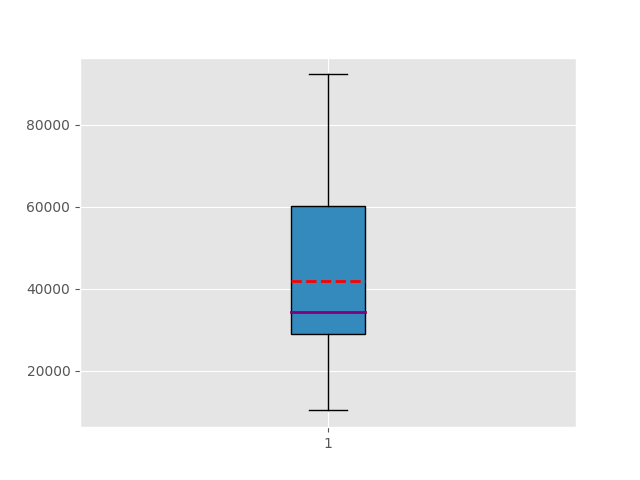
\includegraphics[width=1\textwidth]{Boxplot_NVL.png}
    \caption{NVL stock price's boxplot}
    \label{fig:nvl_boxplot}
    \end{minipage}
    \hfill
    \begin{minipage}{0.23\textwidth}
    \centering
    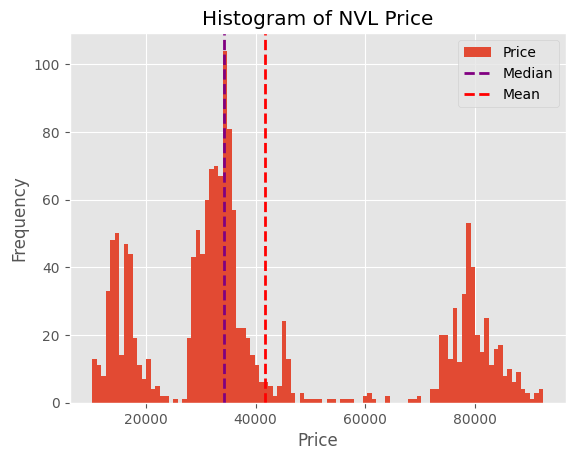
\includegraphics[width=1\textwidth]{Histogram NVL.png}
    \caption{NVL stock price's histogram}
    \label{fig:nvl_histogram}
    \end{minipage}

    \vspace{0.5cm} % Add vertical space between the sets of figures

    \begin{minipage}{0.23\textwidth}
    \centering
    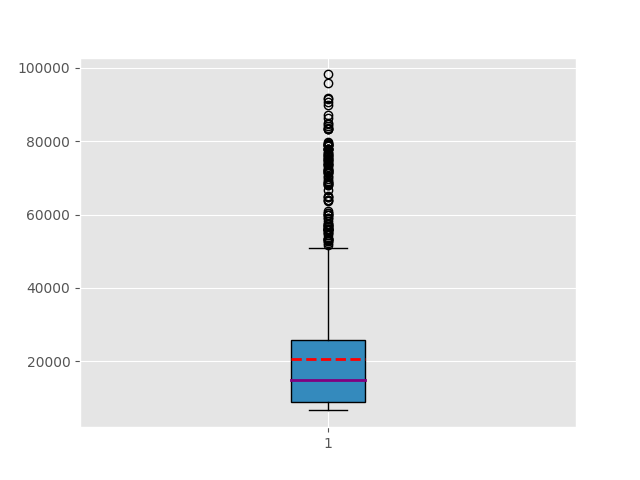
\includegraphics[width=1\textwidth]{Boxplot_DIG.png}
    \caption{DIG stock price's boxplot}
    \label{fig:dig_boxplot}
    \end{minipage}
    \hfill
    \begin{minipage}{0.23\textwidth}
    \centering
    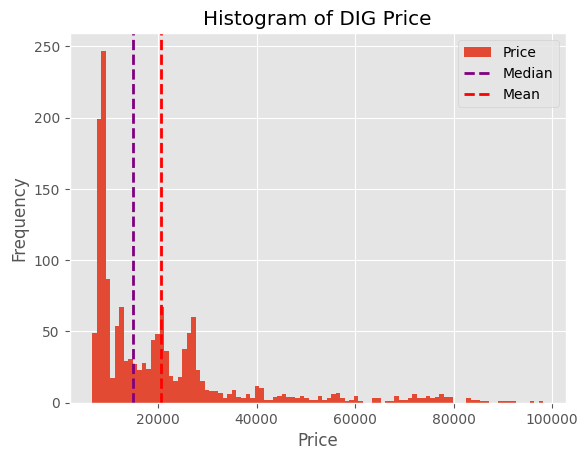
\includegraphics[width=1\textwidth]{Histogram DIG.png}
    \caption{DIG stock price's histogram}
    \label{fig:dig_histogram}
    \end{minipage}

    \vspace{0.5cm} % Add vertical space between the sets of figures

    \begin{minipage}{0.23\textwidth}
    \centering
    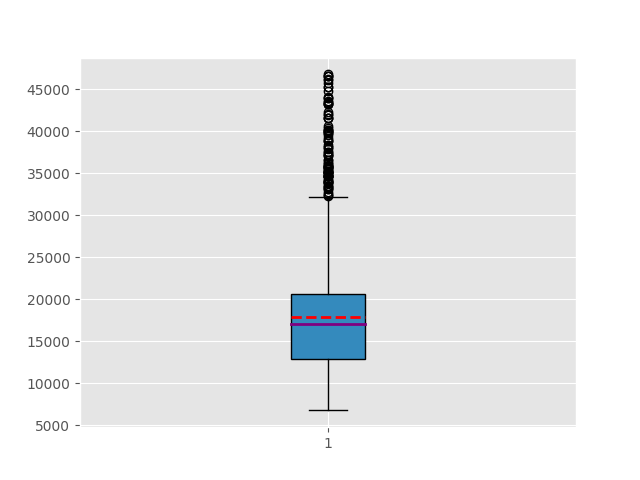
\includegraphics[width=1\textwidth]{Boxplot_DXG.png}
    \caption{DXG stock price's boxplot}
    \label{fig:dxg_boxplot}
    \end{minipage}
    \hfill
    \begin{minipage}{0.23\textwidth}
    \centering
    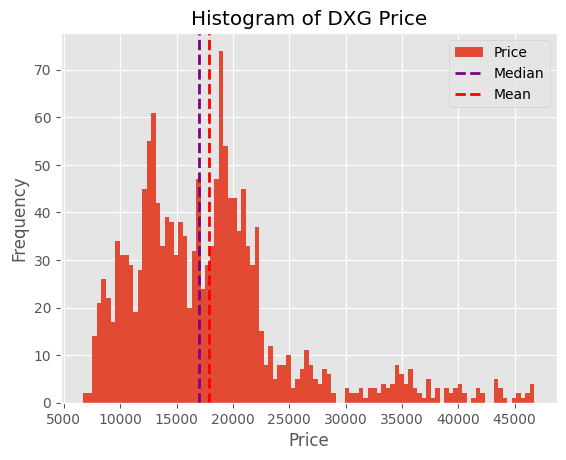
\includegraphics[width=1\textwidth]{Histogram DXG.png}
    \caption{DXG stock price's histogram}
    \label{fig:dxg_histogram}
    \end{minipage}
\end{figure}






\newpage
\section{Methodology}
\subsection{Linear Regression}
Linear regression is a linear approach for modeling the relationship between a scalar response and one or more explanatory variables. In linear regression, the relationships are modeled using linear predictor functions whose unknown model parameters are estimated from the data which are called linear models. Linear regression model follows a very particular form, a regression model is linear when all terms in the model have a constant or a parameter multiplied by an independent variable. And by adding the terms together, the equation is formed:
\[ Y = \beta_0 + \beta_1 X_1 + \beta_2 X_2 + \ldots + \beta_p X_p + \epsilon \]
Where:
\begin{itemize}
    \item $Y$: dependent variable (affected by other variables)
    \item $X_1, X_2, X_p$: independent variables (affecting other variables)
    \item $\beta_0$: regression constant (or intercept). This is the index indicating the value of $Y$ when all $X$ are 0 (no $X$). When represented on the XY graph, $\beta_0$ is the point on the $Oy$ axis where the regression line intersects.
    \item $\beta_1, \beta_2, \beta_p$: regression coefficients, also known as slope coefficients. This index indicates the level of change in $Y$ caused by the corresponding $X$.
    \item $\epsilon$: error term. This index, the larger it is, makes the prediction accuracy of the regression less accurate or more deviated from reality.
\end{itemize}



\subsection{ARIMA}

ARIMA stands for Autoregressive Integrated Moving Average. The ARIMA model is based on the Box and Jenkins method of using three different concepts: autoregressive (AR) model, moving average (MA) model, and integration, together classified as an ARIMA $(p, d, q)$. It is a quantitative forecasting model over time, where the future value of the predictor variable will depend on the movement trend of that object in the past. 
The model contains three components/parameters: AR + I + MA. AR is denoted as $p$, where it shows the weighted linear of sum $p$ values based on ARIMA $(p, d, q)$ terminology. The $p$-value indicates the number of orders. The formula to denote this AR is shown as:

\begin{equation}
\phi_1 = \phi_1 + \phi_2 \delta - \delta x_0 + \phi_3 \delta - \delta x_1 + \ldots + \delta e_{t-1} = e_t
\end{equation}

Where $p$ is used to determine the number of orders of past values; $t$ is the time series; $\phi$ is the coefficient of the AR model; $e$ is the error term with mean zero and variance $\sigma^2$.

MA process is denoted by order $q$ in the ARIMA $(p, d, q)$ classification which shows an error value in Equation (4), it also uses the number of orders in the past values, as denoted in Equation (5)
\begin{equation}
x_t = c +\theta_1 e_{t-1} + \theta_2 e_{t-2} + \ldots + \theta_q e_{t-q} + e_t
\end{equation}
Where $t$ is the time series; $\theta$ is the slope coefficient; $q$ is the number of orders needed to identify the past values. To identify how many orders are in the calculation of AR, the parameter of $q$ is used; c is the intercept

Integrated or differentiated versions are denoted as $d$ in ARIMA $(p, d, q)$, which is the number of times the time series got different.

\begin{equation}
I = \Delta x_t = x_t - x_{t-1}
\end{equation}
Therefore, The ARIMA(p, d, q) can be represented in the following equation:
\begin{equation}
    Y_t = c + \varphi_1 Y_{t-1} + \ldots + \varphi_p Y_{t-p} + \theta_1 \varepsilon_{t-1} + \ldots + \theta_q \varepsilon_{t-q} + \varepsilon_t
\end{equation}

\subsection{ETS}
Exponential smoothing method (ETS) is one of the forecasting model analyses of runtime (time series). This method performs a forecasting approach to the grant of a value weighting over a certain constant on a series of observations of the past to predict future values. This smoothing method adds the parameter alpha (\(\alpha\)) in this model to reduce the factor of randomness \cite{b1}. The exponential term in the weighting is derived from the methods/scales (factor refinement of previous periods that shaped exponential).

Exponential smoothing model variation depending on case data will be foreseen. The following variation of the exponential smoothing model:

\begin{itemize}
    \item Simple Exponential Smoothing (SES): Simple Exponential Smoothing (SES) is a time series forecasting model calculation method that assumes the observation data pattern is stationary tend to straight lines. The formula of the SES is as follows \cite{b2}:
    \[ F_t = \alpha D_t + (1 - \alpha) F_{t-1} \]
    Where:
    \( D_t \) is the actual data value in period \( t \)
    \( F_t \) is forecasting data value on a period \( t \)
    \( \alpha \) is a constant of refinement for the entire data
    
    \item Double Exponential Smoothing (DES): Double Exponential Smoothing (DES) or commonly called Holt's Model is a method of forecasting model calculations that assume the observation data pattern has a trend however no seasonal variations have. This model is also called Trend-Adjusted Exponential Smoothing (TAES) due to an adjustment of the trend on the observation data to influence the accuracy of the results. This method is very good for calculating a linear trend that forecasts short and medium term. The formula of the DES is as follows \cite{b3}:
    \[ F_t = \alpha D_t + (1 - \alpha)(F_{t-1} + T_{t-1}) \]
    \[ T_t = \beta (F_t - F_{t-1}) + (1 - \beta)T_{t-1} \]
    Where:
    \( T_t \) is the trend in the period \( t \)
    \( \beta \) is a constant refinement for trends
    
    \item Triple Exponential Smoothing (TES): Triple Exponential Smoothing (TEST) or commonly called Holt Winters Model is a forecasting model which assumes that the calculation method of observation data has a trend at once seasonal variations. Constant of Gamma (\( \delta \)) is the parameter that controls the weighting observation data for estimating the existence of seasonal variations. Calculation of the TES is almost the same with DES but there is mining of gamma constant value to smooth the seasonal component, with the following calculation formula:
    \[ L_{t} = \alpha \left( \frac{D_{t}}{I_{t-L}} \right) + (1 - \alpha)(L_{t-1} + T_{t-1}) \]
    \[ T_{t} = \beta (L_{t} - L_{t-1}) + (1 - \beta)T_{t-1} \]
    \[ I_{t} = \delta \left( \frac{D_{t}}{L_{t}} \right) + (1 - \delta)I_{t-L} \]
    Where:
    \( I_t \) is the seasonal index in the period \( t \)
    \( \delta \) is a constant smoothing seasonal component
    \( L \) is the length of the season
    
\end{itemize}

The value of alpha, beta, and gamma in the range 0 to 1. The larger the value of the constant, then the greater the weighting towards granting any observation data.
\subsection{Kalman Filter}

Kalman Filter is a Linear-Gaussian State Space Model, a type of time series prediction algorithm, invented by Rudolf Emil Kalman in 1960.\cite{b4}

How Kalman filter works: \\
Initial estimation: Initialize the initial state $\widehat{x}_{0,0}$ and the initial state covariance matrix $P_{0,0}$.\\
Iterative process of prediction and measurement update:

\begin{enumerate}
    \item Prediction
    \begin{itemize}
        \item Prediction of the next state
        \[ \widehat{x}_{n + 1, n} = F\widehat{x}_{n, n} + Gu_{n} \]
        \item Prediction of the next state uncertainty (error)
        \[ P_{n + 1, n} = FP_{n, n}F^{T} + Q \]
    \end{itemize}
    \item Measurement update
    \begin{itemize}
        \item Calculation of the Kalman Gain prediction weight
        \[ K_{n} = P_{n, n - 1}H^{T}(HP_{n, n - 1}H^{T} + R_{n})^{-1} \]
        \item Update of the state estimate
        \[ \widehat{x}_{n, n} = \widehat{x}_{n, n - 1} + K_{n}(Z_{n} - H\widehat{x}_{n, n - 1}) \]
        \item Update of the estimate uncertainty (error)
        \[ P_{n, n} = (1 - K_{n}H)P_{n, n - 1}(1 - K_{n}H)^{T} + K_{n}R_{n}K_{n}^{T} \]
    \end{itemize}

Where:
    \begin{itemize}
        \item $x$: The state actor
        \item $F$: The state transition matrix
        \item $G$: The control matrix
        \item $u$: The input variable
        \item $P$: The covariance matrix
        \item $H$: The observation matrix
        \item ${H}^{T}$: The transpose of the observation matrix
        \item $K$: The Kalman Gain
        \item $R$: The measurement covariance matrix
        \item $z$: The vector measurement
    \end{itemize}
\end{enumerate}

By combining measurement data and prediction models to estimate the state and reduce noise in dynamic systems, Kalman Filter improves the accuracy of the prediction model.
\subsection{TBATS}  
TBATS models are a sophisticated class of time series models that integrate several techniques to address complex data patterns. 

TBATS employs trigonometric functions to model multiple seasonalities simultaneously, such as daily, weekly, and annual cycles. Moreover, a Box-Cox transformation is applied to stabilize the variance, making the data more suitable for modeling.

TBATS models also incorporate ARMA components to manage short-term dynamics and autocorrelations in the residuals, thereby improving forecast accuracy. Additionally, they allow for damping trends, accommodating trends that decrease over time. These features enable TBATS models to effectively handle complex seasonal patterns, nonlinearities, and residual autocorrelations, making them particularly useful for forecasting data with intricate seasonal structures, such as in the case study of forecasting the second wave of the COVID-19 epidemic case study.\cite{b5}

% Dương
\subsection{ResNet}  
ResNet (Residual Network) is a type of deep neural network that utilizes residual blocks to enhance performance and mitigate the vanishing gradient problem as the network becomes very deep. Each residual block comprises three convolutional blocks with different kernel sizes, combined with a shortcut connection that adds the initial input to the final output of the block. This ResNet model includes three residual blocks, followed by a global average pooling layer and a fully connected (fc) layer to produce the final output. \cite{b6}

\begin{enumerate}
  \item Equations
  
  Assume $x$ is the initial input of the residual block. Each convolutional block performs the following transformations:
  \begin{align*}
    h_1 &= \text{ReLU}(\text{BN}(\text{Conv1d}(x))) \\
    h_2 &= \text{ReLU}(\text{BN}(\text{Conv1d}(h_1))) \\
    h_3 &= \text{BN}(\text{Conv1d}(h_2))
  \end{align*}

  The output of the residual block is calculated by adding the initial input $x$ to $h_3$ and then applying the ReLU function:
  \begin{align*}
    y &= h_3 + x \\
    \hat{h} &= \text{ReLU}(y)
  \end{align*}

  The number of filters for the residual blocks is $k_i = \{64, 128, 128\}$.

  \vspace{0.5cm}  % Optional vertical spacing

  ResNet Structure:

  The ResNet structure is as follows: \\
  \begin{align*}
    \text{ResNet} &= [\text{ResBlock1}, \text{ResBlock2}, \\
                    &\quad \text{ResBlock3}, \text{GlobalAvgPooling}, \text{FC}] \cite{b6}
  \end{align*}
    
  \item ResNetLSTM
  
    ResNetLSTM combines the ResNet architecture with LSTM (Long Short-Term Memory) to handle time series data. After the inputs are processed through the three residual blocks of ResNet, the output is transformed to be suitable for the LSTM input. LSTM has the ability to remember information across time steps, making the model better suited for handling time series data. Finally, a fully connected layer is used to produce the final output. \cite{b7} \\ 
    The output of ResNet is calculated as described above. The output from the last residual block is transformed to fit the LSTM input:

    \begin{align*}
        x_{\text{lstm}} = x.\text{transpose}(1, 2)
    \end{align*}
    
    The LSTM processes the input and returns the output at the last time step:
    \begin{align*}
      x_{\text{lstm}}, (h_n, c_n) = \text{LSTM}(x_{\text{lstm}})
    \end{align*}
    \begin{align*}
      x_{\text{final}} = x_{\text{lstm}}[:, -1, :]
    \end{align*}
    The final output is computed by the fully connected layer:    \begin{align*}
      y = \text{FC}(x_{\text{final}})
    \end{align*}

     
     The ResNetLSTM structure is as follows: 
     \begin{align*}
        \text{ResNetLSTM} = [\text{ResBlock1}, \text{ResBlock2},\\ \text{ResBlock3}, \text{LSTM}, \text{FC}]
    \end{align*}
  \item Summary \\
    ResNet focuses on using residual blocks to increase the depth of the neural network and mitigate the vanishing gradient problem. ResNetLSTM combines the power of ResNet in handling spatial features with the capability of LSTM in remembering and processing temporal features.\\
    The main difference between the two models lies in the final part of each model:
    \subsubsection{ResNet}
    \begin{itemize}
      \item Uses a global average pooling layer: \\
        \text{self.global\_avg\_pool} = \text{nn.AdaptiveAvgPool1d}(1)
      \item The output from the global average pooling layer is fed into the fully connected layer: \\
        $x = \text{self.fc}(x)$
    \end{itemize}
    
    \subsubsection{ResNetLSTM}
    \begin{itemize}
      \item Uses an LSTM layer: 
        \begin{align*}
          \text{self.lstm} &= \text{nn.LSTM}(nf \times 2, \text{lstm\_hidden\_units}, \\
                                          &\quad \text{num\_lstm\_layers}, \text{batch\_first=True})
        \end{align*}
      \item The output from the LSTM is taken at the last time step and fed into the fully connected layer: 
        \begin{align*}
          x &= x[:, -1, :] \\
          x &= \text{self.fc}(x)
        \end{align*}
    \end{itemize}

\end{enumerate}




\section{Experiment}

\begin{figure}[htbp]
\subsection{ARIMA}
\centering
    \begin{minipage}{0.23\textwidth}
    \centering
    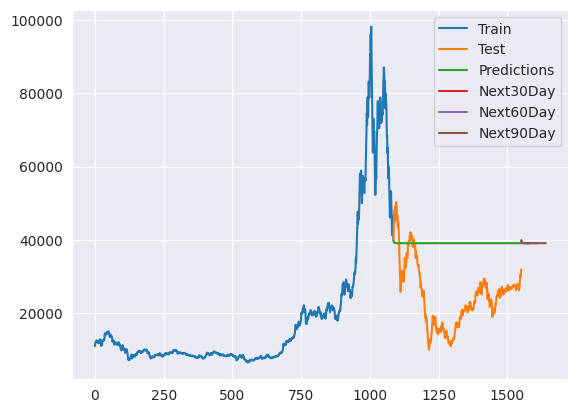
\includegraphics[width=1\textwidth]{experiment/arima/DIG/7 _ 3/7_3_train_test_DIG_ARIMA_plot.png}
    \caption{ARIMA DIG 7-3}
    \label{fig:nvl_boxplot}
    \end{minipage}
    \hfill
    \begin{minipage}{0.23\textwidth}
    \centering
    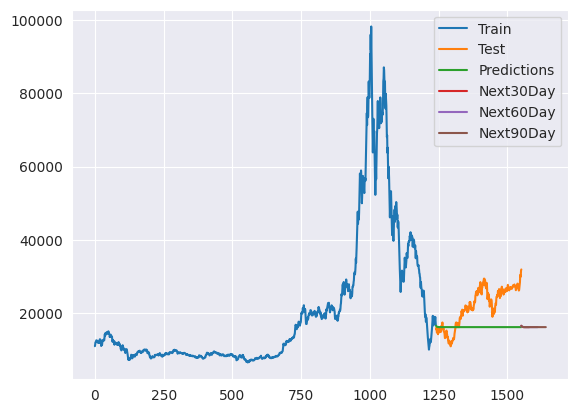
\includegraphics[width=1\textwidth]{experiment/arima/DIG/8 _ 2/8_2_train_test_DIG_ARIMA_plot.png}
    \caption{ARIMA DIG 8-2}
    \label{fig:nvl_histogram}
    \end{minipage}
    \begin{minipage}{0.23\textwidth}
    \centering
    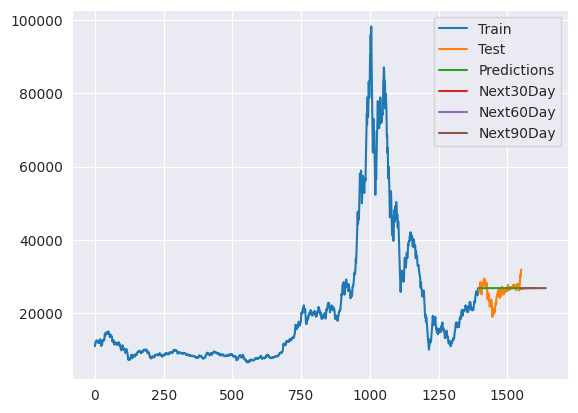
\includegraphics[width=1\textwidth]{experiment/arima/DIG/9 _ 1/9_1_train_test_DIG_ARIMA_plot.png}
    \caption{ARIMA DIG 9-1}
    \label{fig:nvl_histogram}
    \end{minipage}

    \vspace{0.5cm} % Add vertical space between the sets of figures

    \begin{minipage}{0.23\textwidth}
    \centering
    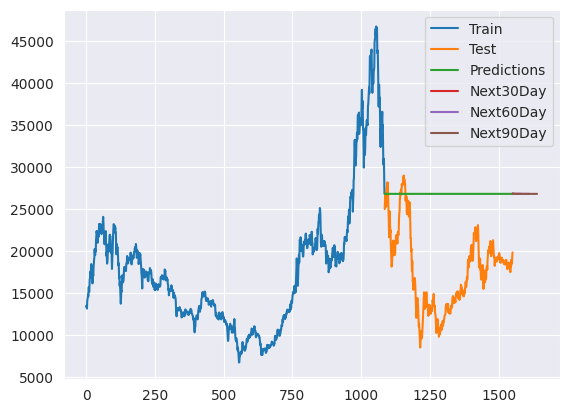
\includegraphics[width=1\textwidth]{experiment/arima/DXG/7 _ 3/7_3_train_test_DXG_ARIMA_plot.png}
    \caption{ARIMA DXG 7-3}
    \label{fig:nvl_boxplot}
    \end{minipage}
    \hfill
    \begin{minipage}{0.23\textwidth}
    \centering
    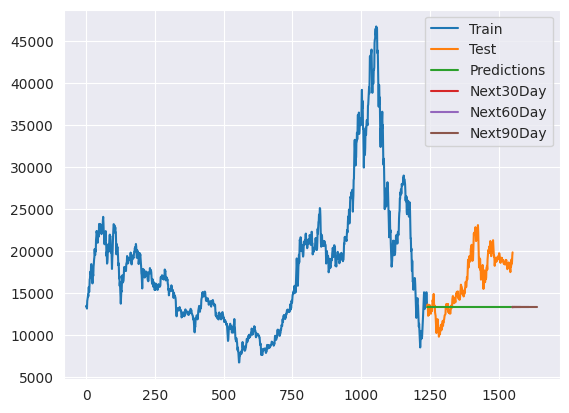
\includegraphics[width=1\textwidth]{experiment/arima/DXG/8 _ 2/8_2_train_test_DXG_ARIMA_plot.png}
    \caption{ARIMA DXG 8-2}
    \label{fig:nvl_histogram}
    \end{minipage}
    \begin{minipage}{0.23\textwidth}
    \centering
    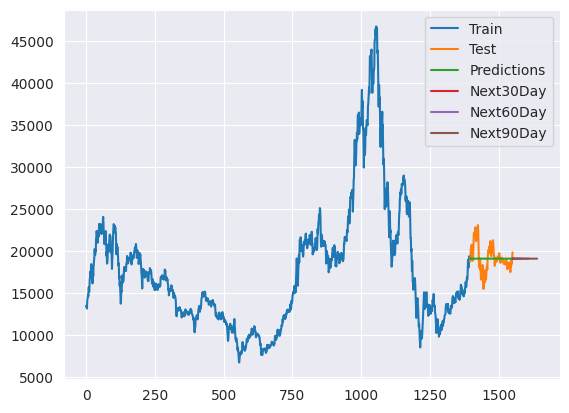
\includegraphics[width=1\textwidth]{experiment/arima/DXG/9 _ 1/9_1_train_test_DXG_ARIMA_plot.png}
    \caption{ARIMA DXG 9-1}
    \label{fig:nvl_histogram}
    \end{minipage}

    \begin{minipage}{0.23\textwidth}
    \centering
    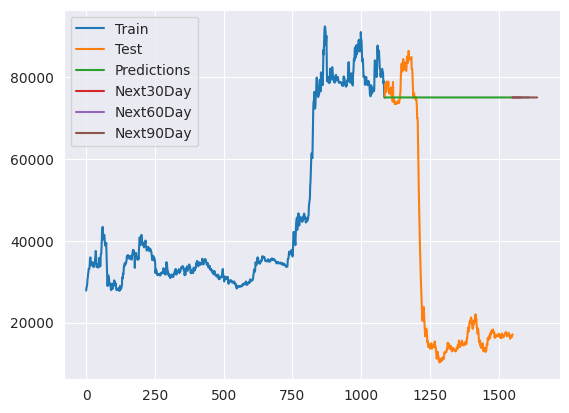
\includegraphics[width=1\textwidth]{experiment/arima/NVL/7 _ 3/7_3_train_test_NVL_ARIMA_plot.png}
    \caption{ARIMA NVL 7-3}
    \label{fig:nvl_boxplot}
    \end{minipage}
    \hfill
    \begin{minipage}{0.23\textwidth}
    \centering
    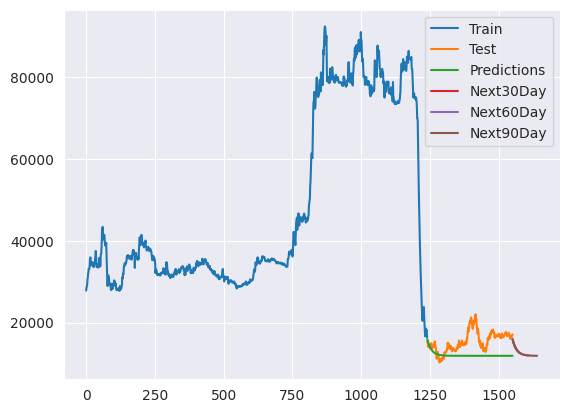
\includegraphics[width=1\textwidth]{experiment/arima/NVL/8 _ 2/8_2_train_test_NVL_ARIMA_plot.png}
    \caption{ARIMA NVL 8-2}
    \label{fig:nvl_histogram}
    \end{minipage}
    \begin{minipage}{0.23\textwidth}
    \centering
    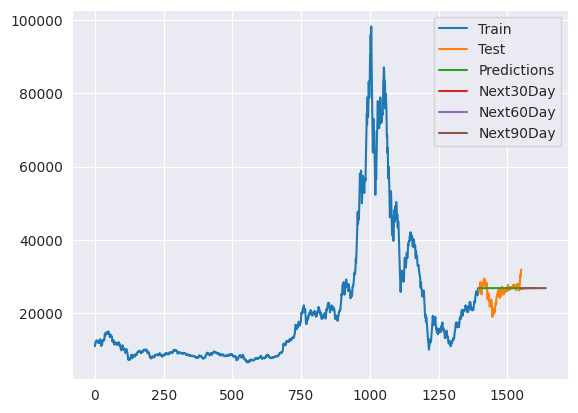
\includegraphics[width=1\textwidth]{experiment/arima/DIG/9 _ 1/9_1_train_test_DIG_ARIMA_plot.png}
    \caption{ARIMA NVL 9-1}
    \label{fig:nvl_histogram}
    \end{minipage}
\end{figure}

\begin{figure}[htbp]
\subsection{ETS}
\centering
    \begin{minipage}{0.23\textwidth}
    \centering
    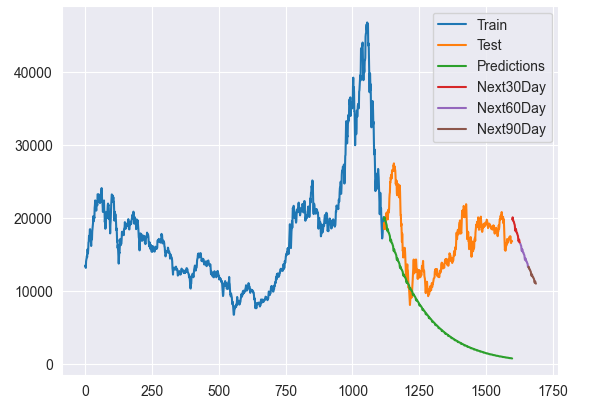
\includegraphics[width=1\textwidth]{experiment/ets/TEAM4_ETS_DIG_7_3.png}
    \caption{ETS DIG 7-3}
    \label{fig:nvl_boxplot}
    \end{minipage}
    \hfill
    \begin{minipage}{0.23\textwidth}
    \centering
    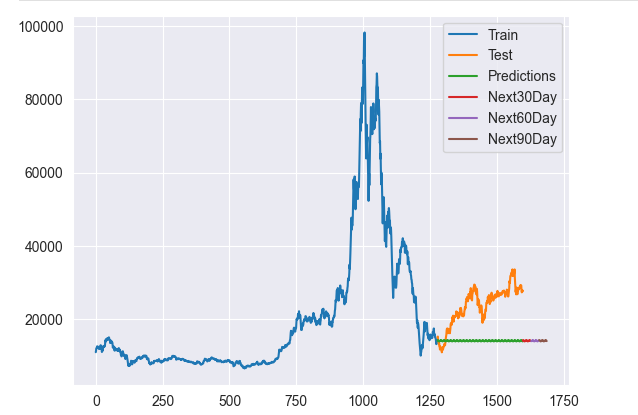
\includegraphics[width=1\textwidth]{experiment/ets/TEAM4_ETS_DIG_8_2.png}
    \caption{ETS DIG 8-2}
    \label{fig:nvl_histogram}
    \end{minipage}
    \begin{minipage}{0.23\textwidth}
    \centering
    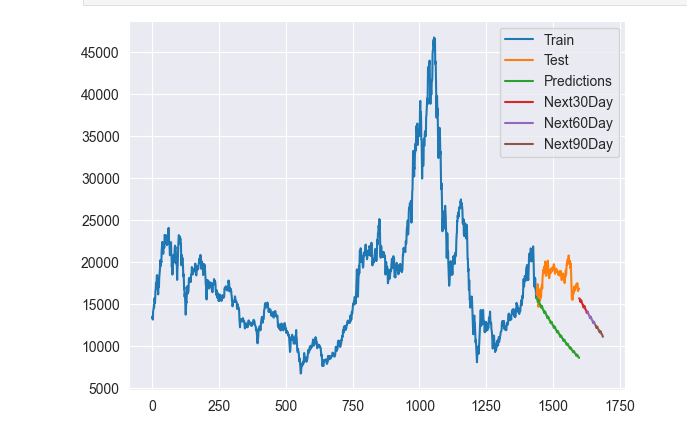
\includegraphics[width=1\textwidth]{experiment/ets/TEAM4_ETS_DIG_9_1.png}
    \caption{ETS DIG 9-1}
    \label{fig:nvl_histogram}
    \end{minipage}

    \vspace{0.5cm} % Add vertical space between the sets of figures

    \begin{minipage}{0.23\textwidth}
    \centering
    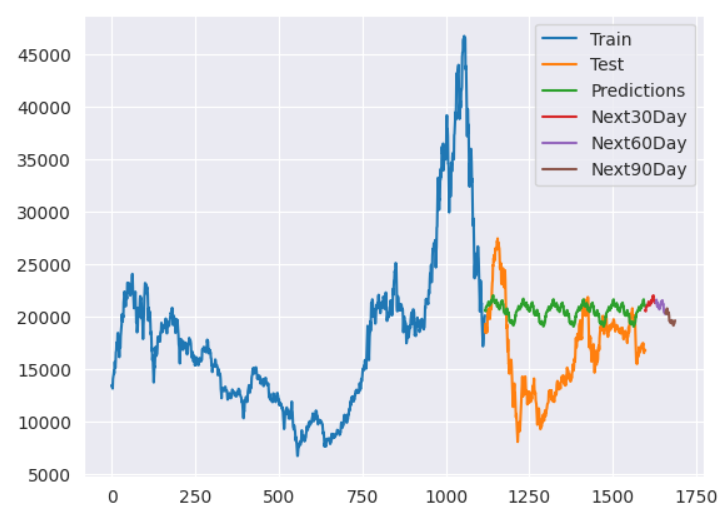
\includegraphics[width=1\textwidth]{experiment/ets/TEAM4_ETS_DXG_7_3.png}
    \caption{ETS DXG 7-3}
    \label{fig:nvl_boxplot}
    \end{minipage}
    \hfill
    \begin{minipage}{0.23\textwidth}
    \centering
    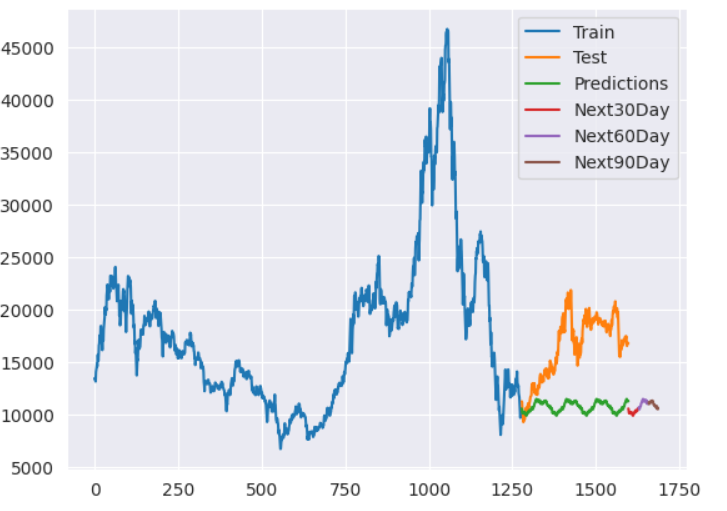
\includegraphics[width=1\textwidth]{experiment/ets/TEAM4_ETS_DXG_8_2.png}
    \caption{ETS DXG 8-2}
    \label{fig:nvl_histogram}
    \end{minipage}
    \begin{minipage}{0.23\textwidth}
    \centering
    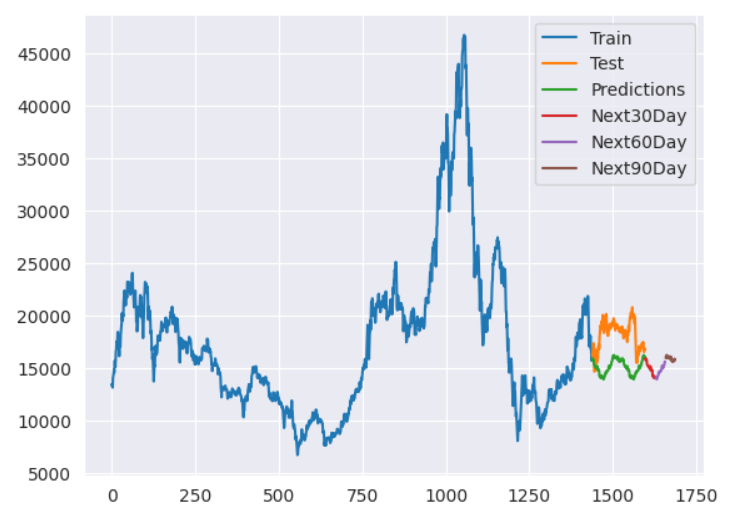
\includegraphics[width=1\textwidth]{experiment/ets/TEAM4_ETS_DXG_9_1.png}
    \caption{ETS DXG 9-1}
    \label{fig:nvl_histogram}
    \end{minipage}

    \begin{minipage}{0.23\textwidth}
    \centering
    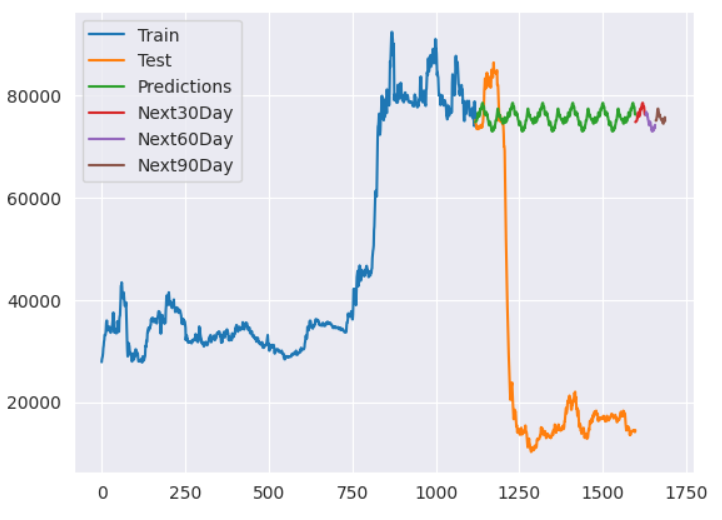
\includegraphics[width=1\textwidth]{experiment/ets/TEAM4_ETS_NVL_7_3.png}
    \caption{ETS NVL 7-3}
    \label{fig:nvl_boxplot}
    \end{minipage}
    \hfill
    \begin{minipage}{0.23\textwidth}
    \centering
    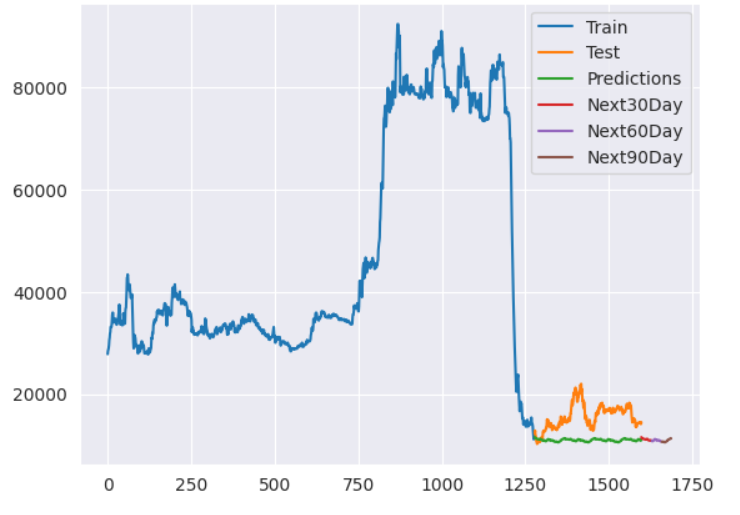
\includegraphics[width=1\textwidth]{experiment/ets/TEAM4_ETS_NVL_8_2.png}
    \caption{ETS NVL 8-2}
    \label{fig:nvl_histogram}
    \end{minipage}
    \begin{minipage}{0.23\textwidth}
    \centering
    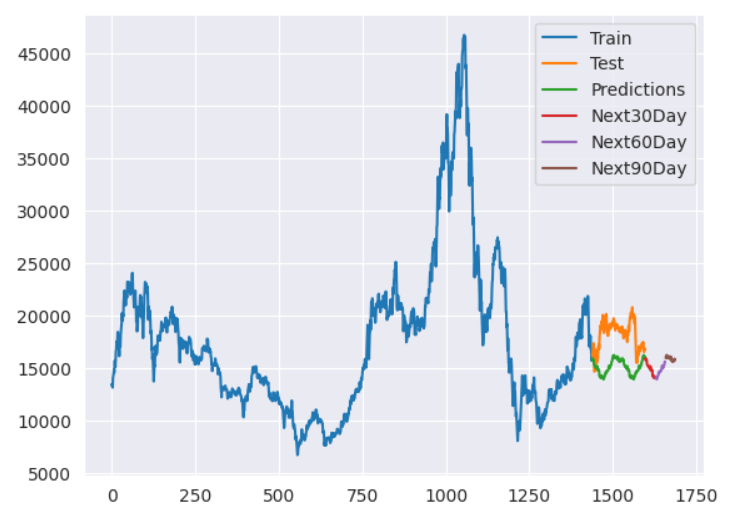
\includegraphics[width=1\textwidth]{experiment/ets/TEAM4_ETS_DXG_9_1.png}
    \caption{ETS NVL 9-1}
    \label{fig:nvl_histogram}
    \end{minipage}
\end{figure}
\newpage


\begin{figure}[htbp]
\subsection{Kalman Filter}
\centering
    \begin{minipage}{0.23\textwidth}
    \centering
    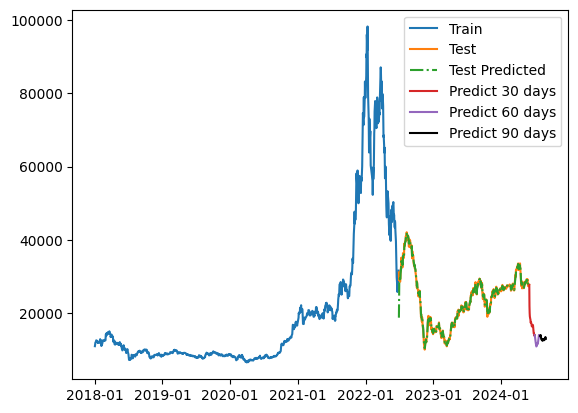
\includegraphics[width=1\textwidth]{experiment/kf/DIG 7-3.png}
    \caption{Kalman Filter DIG 7-3}
    \label{fig:nvl_boxplot}
    \end{minipage}
    \hfill
    \begin{minipage}{0.23\textwidth}
    \centering
    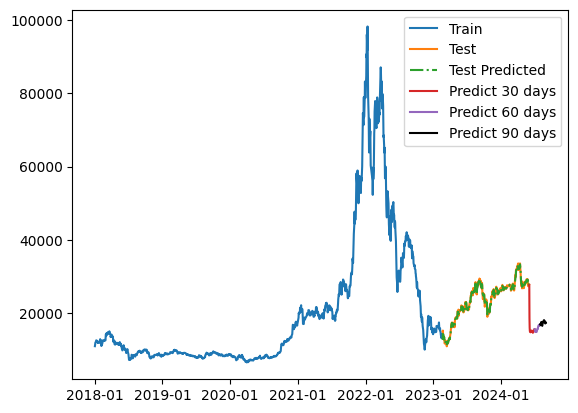
\includegraphics[width=1\textwidth]{experiment/kf/dig 8-2.png}
    \caption{Kalman Filter DIG 8-2}
    \label{fig:nvl_histogram}
    \end{minipage}
    \begin{minipage}{0.23\textwidth}
    \centering
    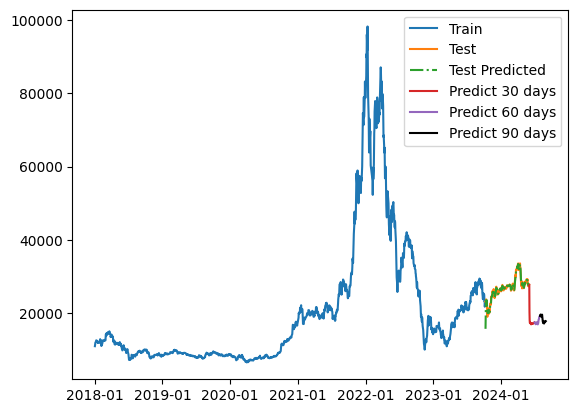
\includegraphics[width=1\textwidth]{experiment/kf/DIG 9-1.png}
    \caption{Kalman Filter DIG 9-1}
    \label{fig:nvl_histogram}
    \end{minipage}

    \vspace{0.5cm} % Add vertical space between the sets of figures

    \begin{minipage}{0.23\textwidth}
    \centering
    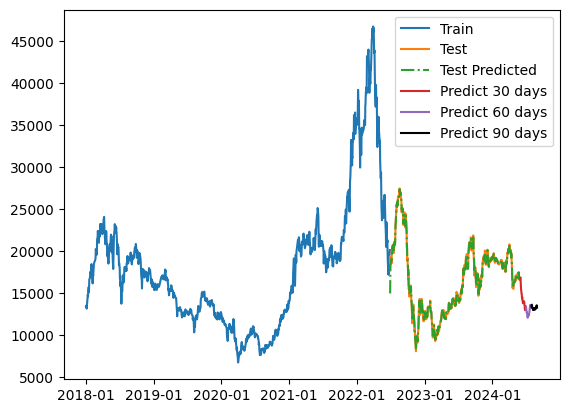
\includegraphics[width=1\textwidth]{experiment/kf/DXG 7-3.png}
    \caption{Kalman Filter DXG 7-3}
    \label{fig:nvl_boxplot}
    \end{minipage}
    \hfill
    \begin{minipage}{0.23\textwidth}
    \centering
    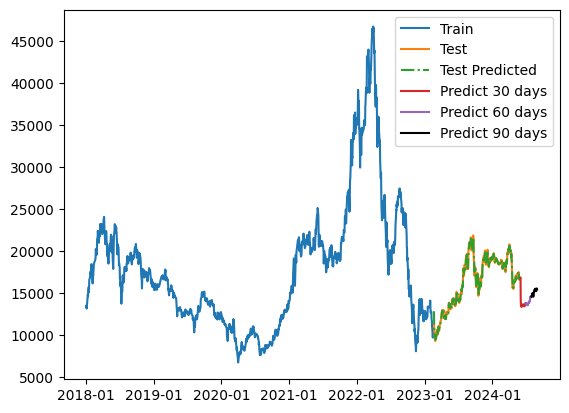
\includegraphics[width=1\textwidth]{experiment/kf/DXG 8-2.png}
    \caption{Kalman Filter DXG 8-2}
    \label{fig:nvl_histogram}
    \end{minipage}
    \begin{minipage}{0.23\textwidth}
    \centering
    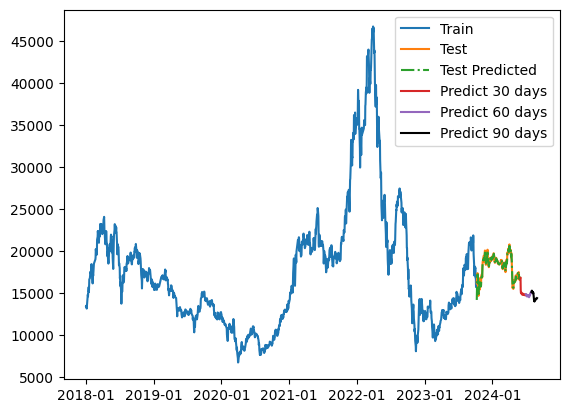
\includegraphics[width=1\textwidth]{experiment/kf/DXG 9-1.png}
    \caption{Kalman Filter DXG 9-1}
    \label{fig:nvl_histogram}
    \end{minipage}

    \begin{minipage}{0.23\textwidth}
    \centering
    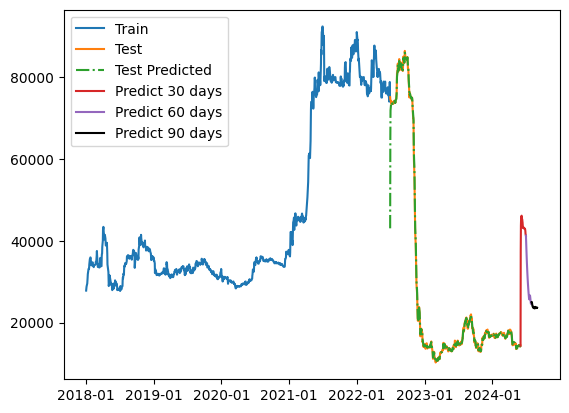
\includegraphics[width=1\textwidth]{experiment/kf/NVL 7-3.png}
    \caption{Kalman Filter NVL 7-3}
    \label{fig:nvl_boxplot}
    \end{minipage}
    \hfill
    \begin{minipage}{0.23\textwidth}
    \centering
    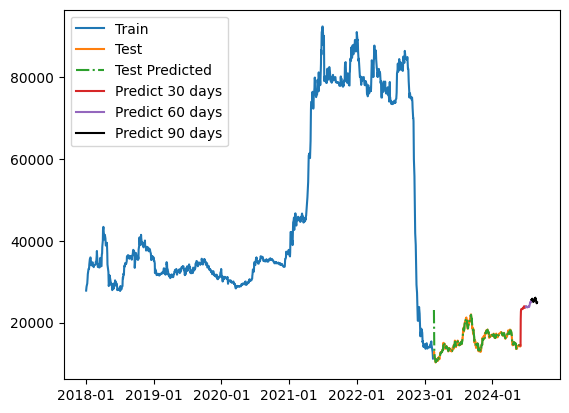
\includegraphics[width=1\textwidth]{experiment/kf/NVL 8-2.png}
    \caption{Kalman Filter NVL 8-2}
    \label{fig:nvl_histogram}
    \end{minipage}
    \begin{minipage}{0.23\textwidth}
    \centering
    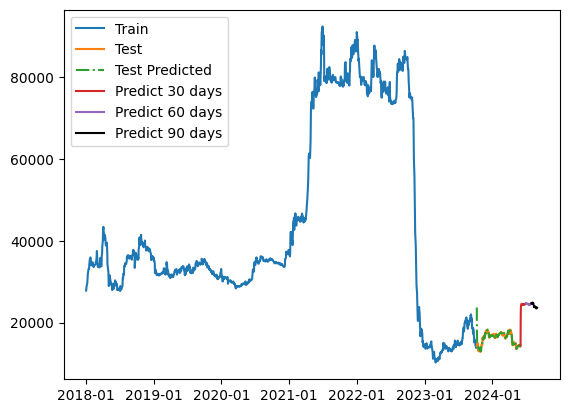
\includegraphics[width=1\textwidth]{experiment/kf/NVL 9-1.png}
    \caption{Kalman Filter NVL 9-1}
    \label{fig:nvl_histogram}
    \end{minipage}
\end{figure}


\begin{figure}[htbp]
\subsection{Resnet}
\centering
    \begin{minipage}{0.23\textwidth}
    \centering
    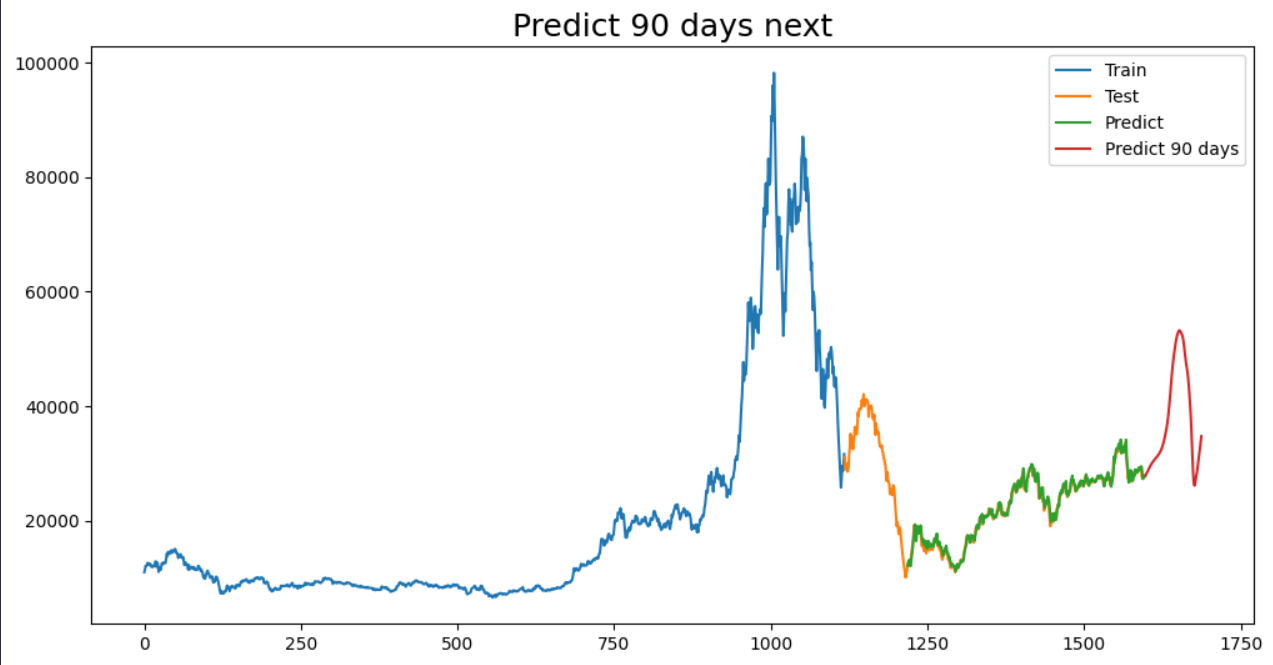
\includegraphics[width=1\textwidth]{experiment/resnet/DIG 7_3.png}
    \caption{ResNet DIG 7-3}
    \label{fig:nvl_boxplot}
    \end{minipage}
    \hfill
    \begin{minipage}{0.23\textwidth}
    \centering
    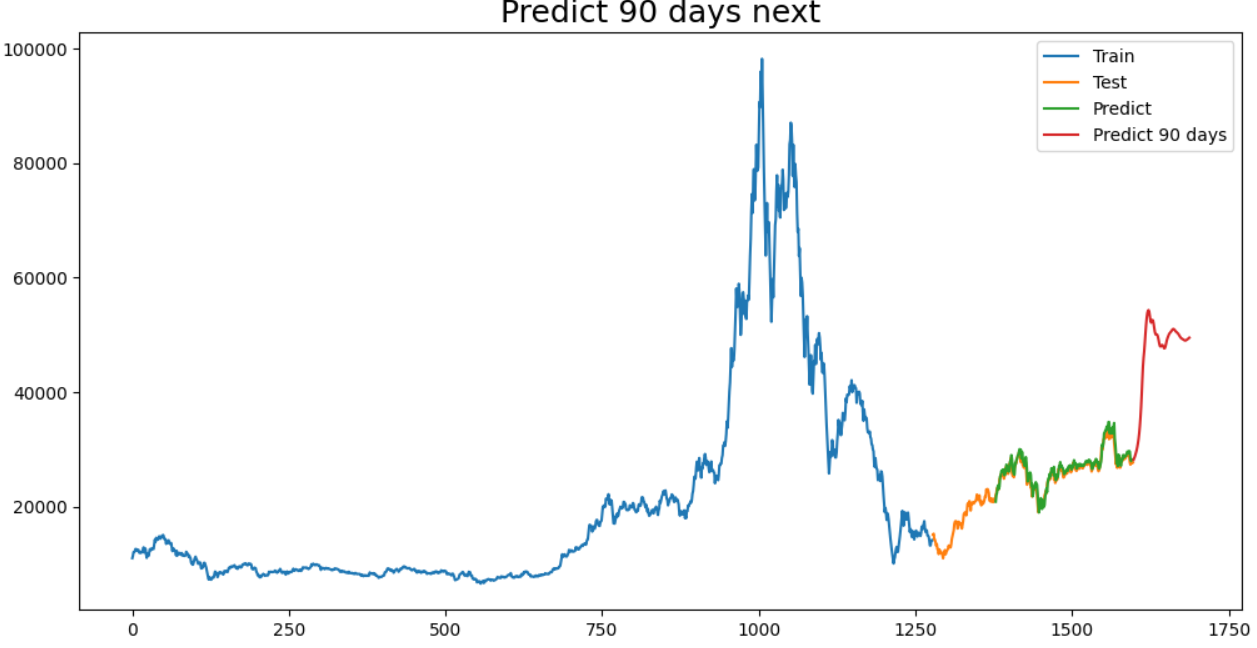
\includegraphics[width=1\textwidth]{experiment/resnet/DIG 8_2.png}
    \caption{ResNet DIG 8-2}
    \label{fig:nvl_histogram}
    \end{minipage}
    \begin{minipage}{0.23\textwidth}
    \centering
    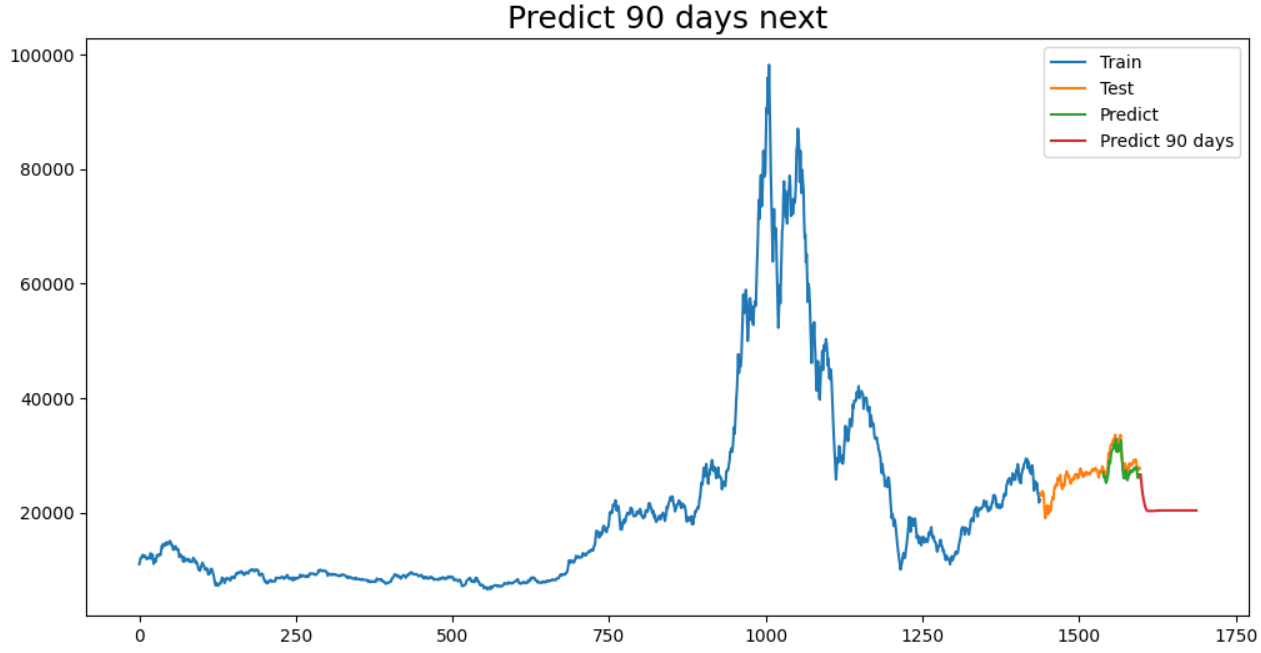
\includegraphics[width=1\textwidth]{experiment/resnet/DIG 9_1.png}
    \caption{ResNet DIG 9-1}
    \label{fig:nvl_histogram}
    \end{minipage}

    \vspace{0.5cm} % Add vertical space between the sets of figures

    \begin{minipage}{0.23\textwidth}
    \centering
    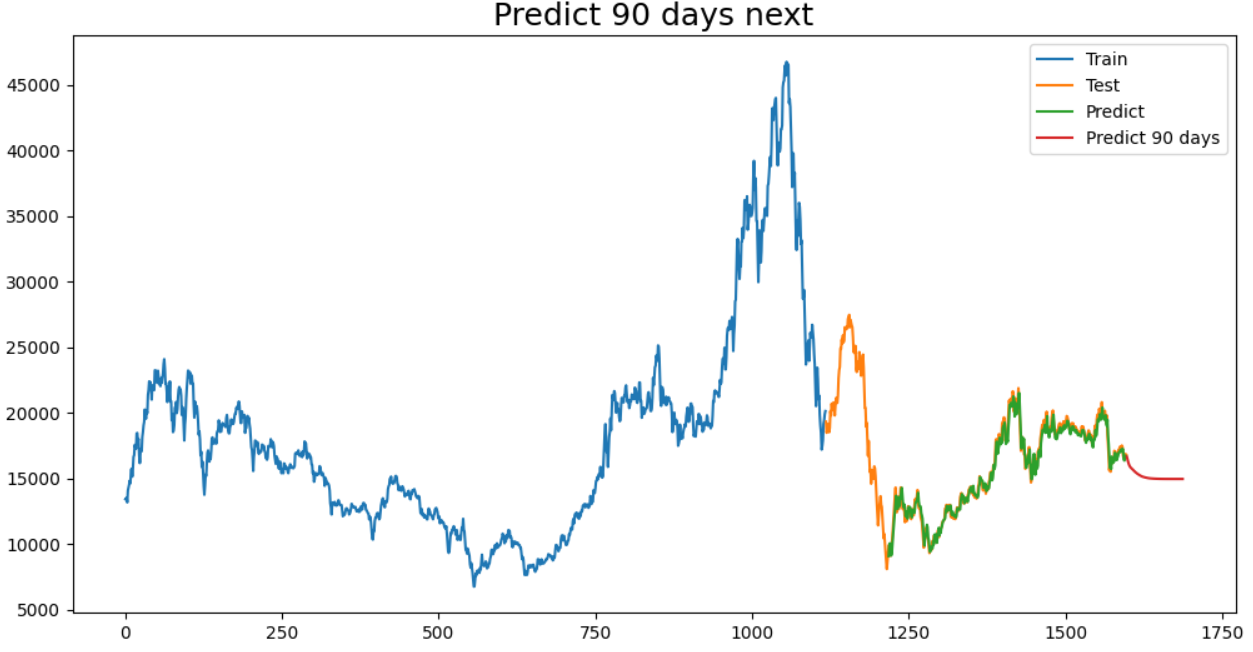
\includegraphics[width=1\textwidth]{experiment/resnet/DXG 7_3.png}
    \caption{ResNet DXG 7-3}
    \label{fig:nvl_boxplot}
    \end{minipage}
    \hfill
    \begin{minipage}{0.23\textwidth}
    \centering
    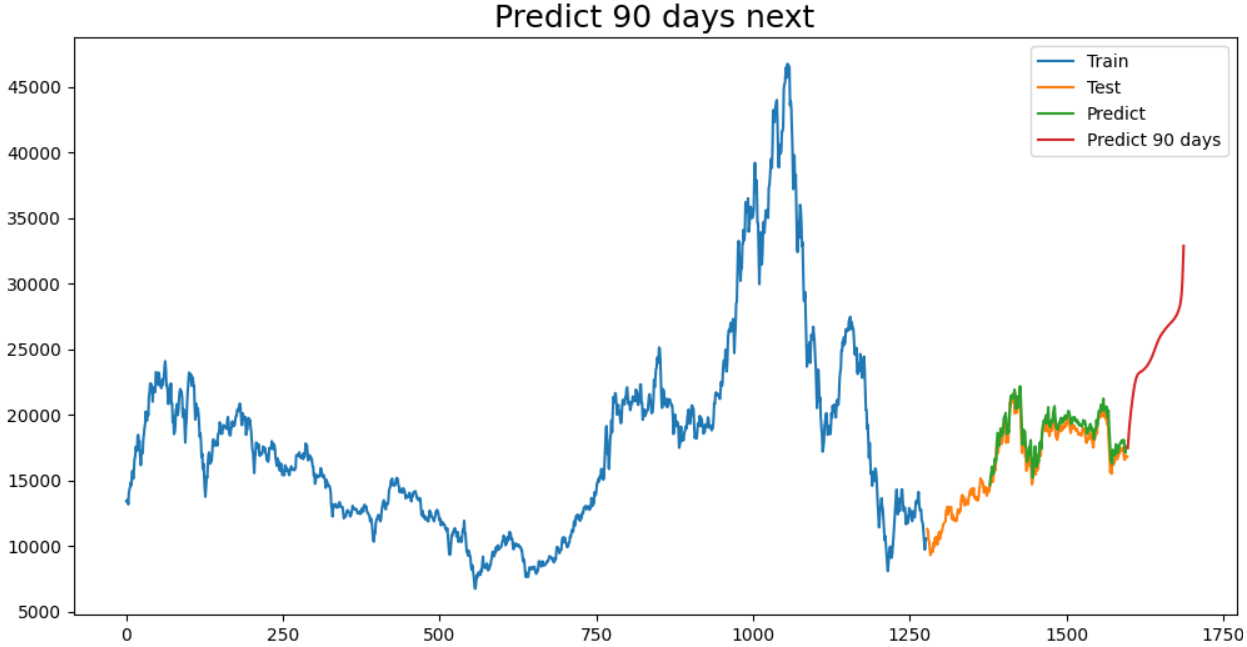
\includegraphics[width=1\textwidth]{experiment/resnet/DXG 8_2.png}
    \caption{ResNet DXG 8-2}
    \label{fig:nvl_histogram}
    \end{minipage}
    \begin{minipage}{0.23\textwidth}
    \centering
    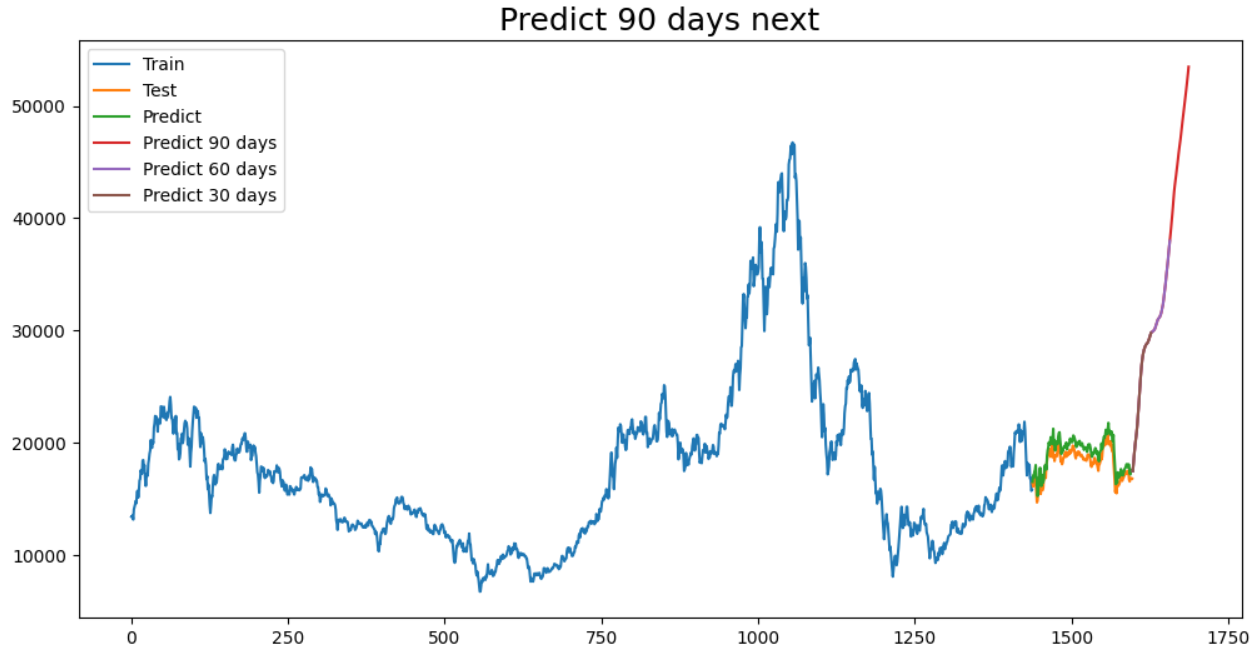
\includegraphics[width=1\textwidth]{experiment/resnet/DXG 9_1.png}
    \caption{ResNet DXG 9-1}
    \label{fig:nvl_histogram}
    \end{minipage}

    \begin{minipage}{0.23\textwidth}
    \centering
    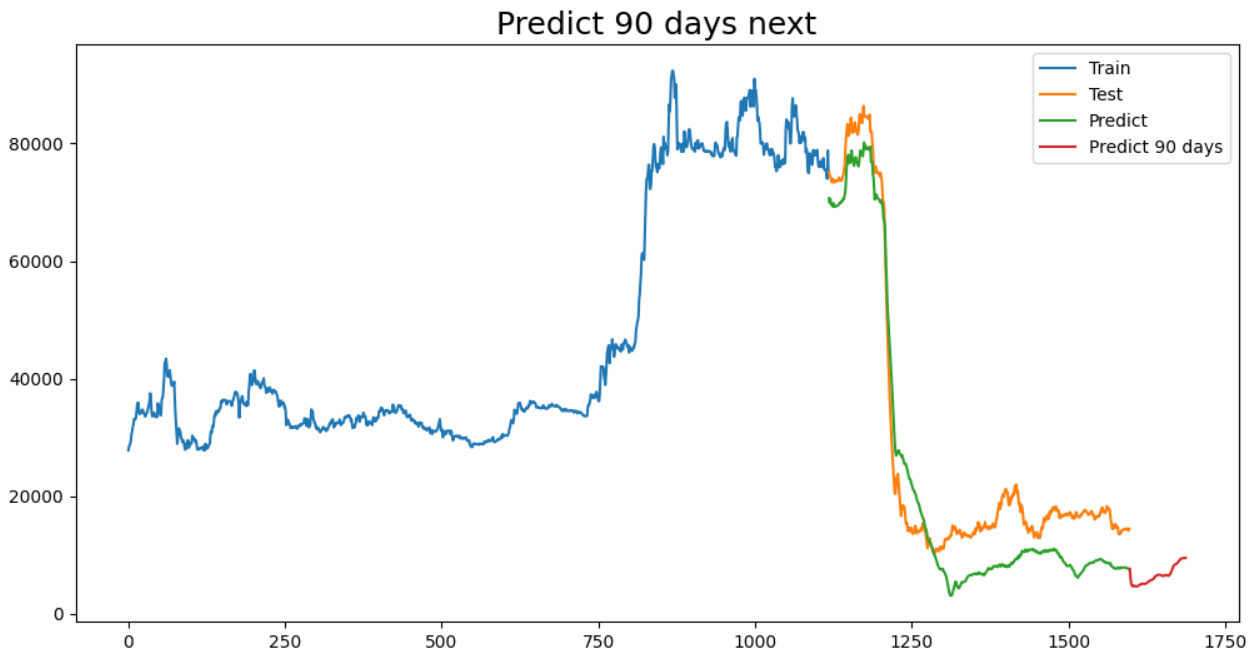
\includegraphics[width=1\textwidth]{experiment/resnet/NVL 7_3.png}
    \caption{ResNet NVL 7-3}
    \label{fig:nvl_boxplot}
    \end{minipage}
    \hfill
    \begin{minipage}{0.23\textwidth}
    \centering
    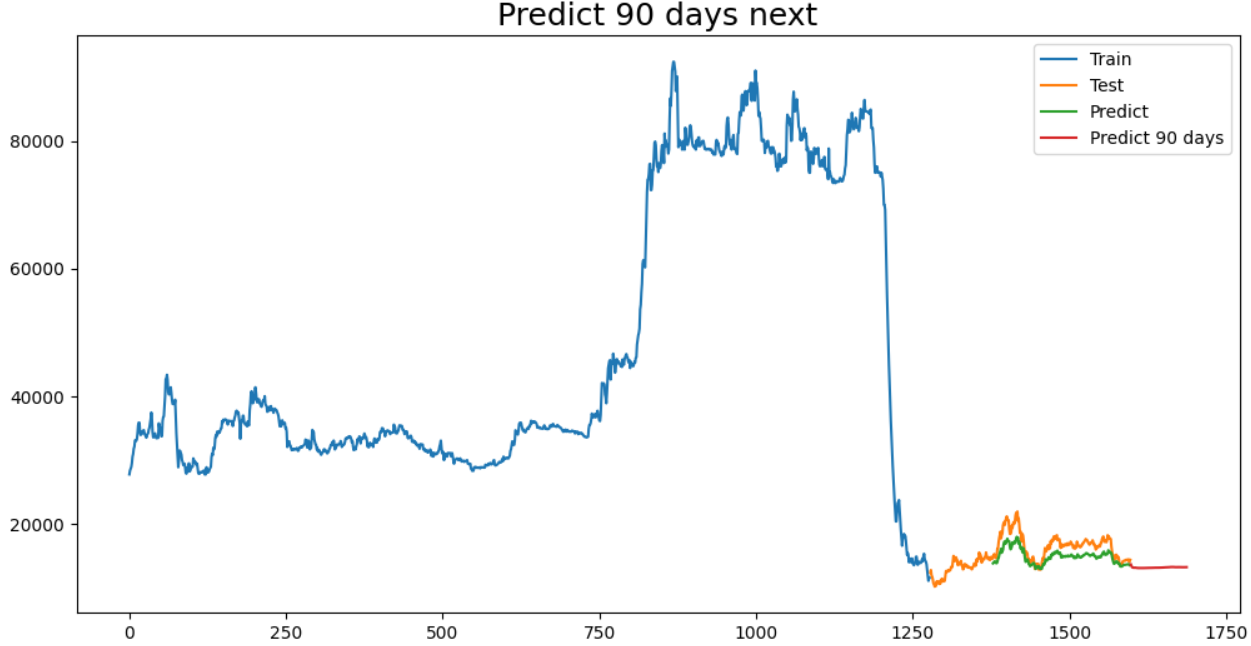
\includegraphics[width=1\textwidth]{experiment/resnet/NVL 8_2.png}
    \caption{ResNet NVL 8-2}
    \label{fig:nvl_histogram}
    \end{minipage}
    \begin{minipage}{0.23\textwidth}
    \centering
    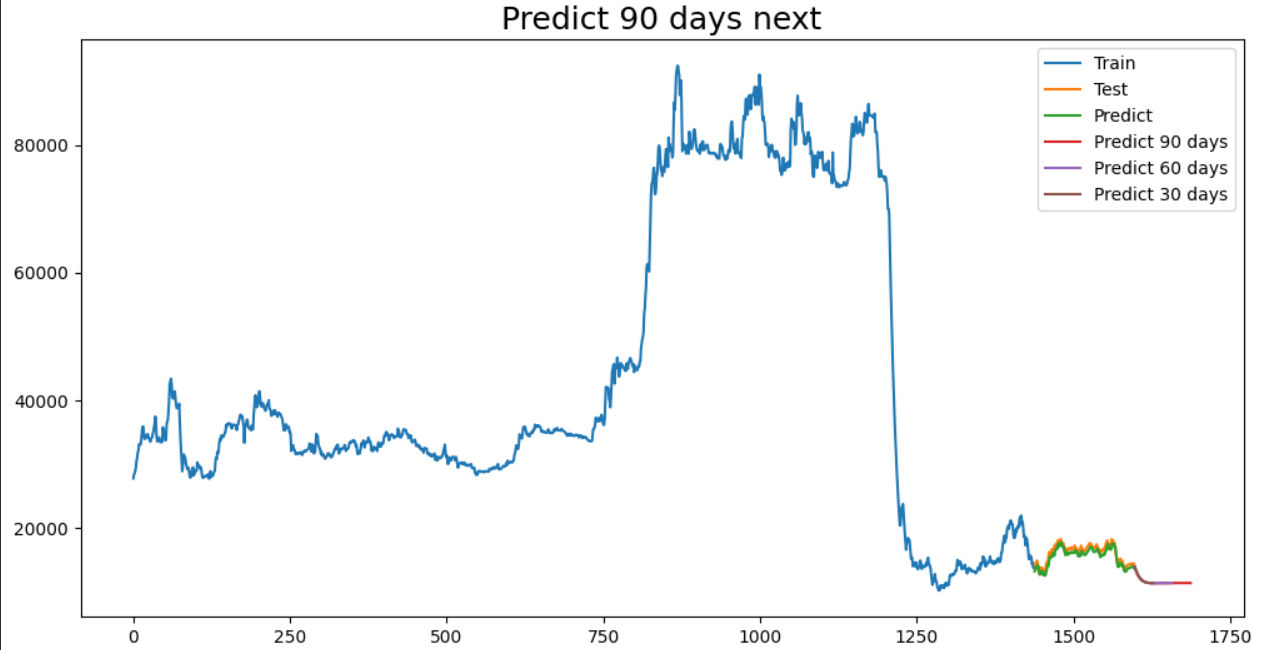
\includegraphics[width=1\textwidth]{experiment/resnet/NVL 9_1.png}
    \caption{ResNet NVL 9-1}
    \label{fig:nvl_histogram}
    \end{minipage}
\end{figure}


\begin{figure}[htbp]
\subsection{LSTM}
\centering
    \begin{minipage}{0.23\textwidth}
    \centering
    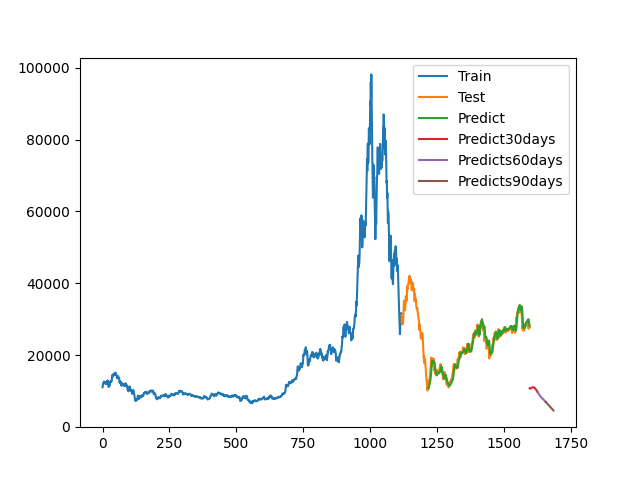
\includegraphics[width=1\textwidth]{experiment/ltsm/Team4_LSTM_DIG_7_3.png}
    \caption{LSTM DIG 7-3}
    \label{fig:nvl_boxplot}
    \end{minipage}
    \hfill
    \begin{minipage}{0.23\textwidth}
    \centering
    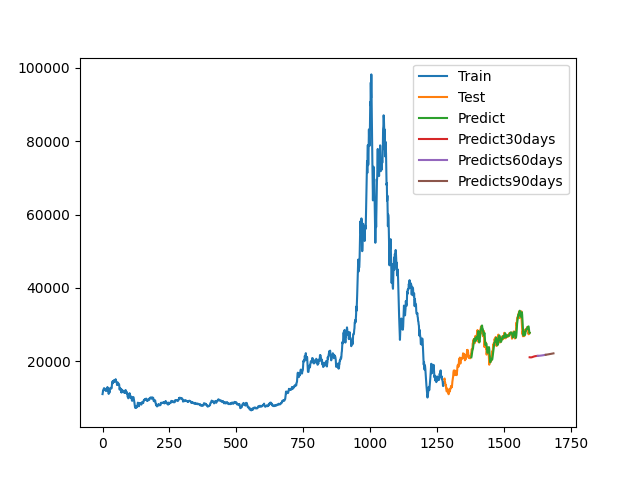
\includegraphics[width=1\textwidth]{experiment/ltsm/Team4_LSTM_DIG_8_2.png}
    \caption{LSTM DIG 8-2}
    \label{fig:nvl_histogram}
    \end{minipage}
    \begin{minipage}{0.23\textwidth}
    \centering
    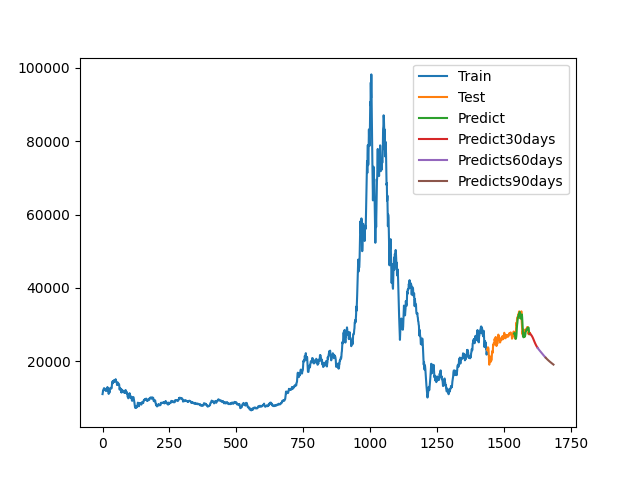
\includegraphics[width=1\textwidth]{experiment/ltsm/Team4_LSTM_DIG_9_1.png}
    \caption{LSTM DIG 9-1}
    \label{fig:nvl_histogram}
    \end{minipage}

    \vspace{0.5cm} % Add vertical space between the sets of figures

    \begin{minipage}{0.23\textwidth}
    \centering
    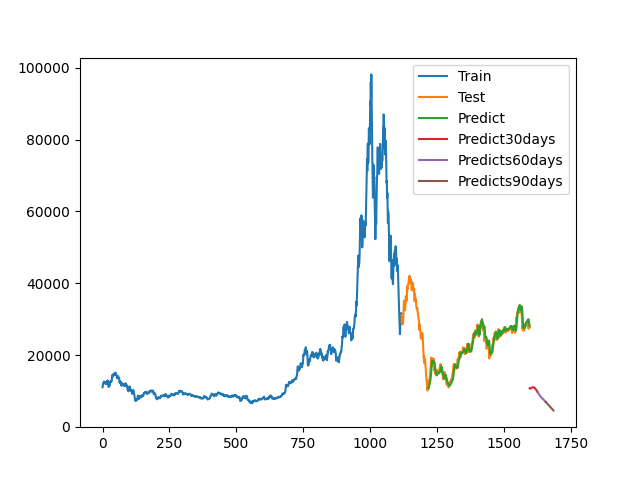
\includegraphics[width=1\textwidth]{experiment/ltsm/Team4_LSTM_DIG_7_3.png}
    \caption{LSTM DXG 7-3}
    \label{fig:nvl_boxplot}
    \end{minipage}
    \hfill
    \begin{minipage}{0.23\textwidth}
    \centering
    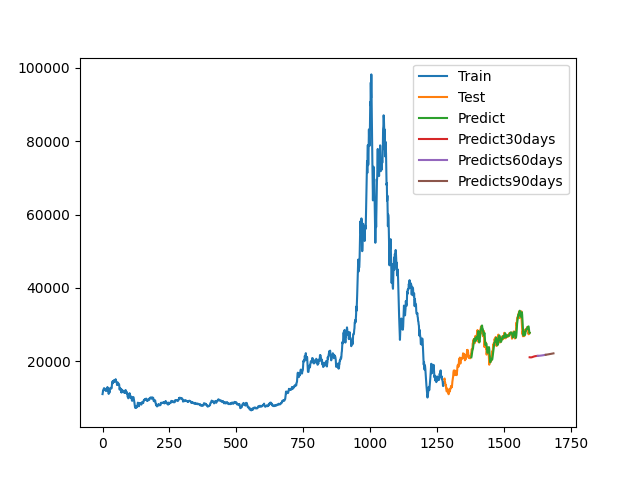
\includegraphics[width=1\textwidth]{experiment/ltsm/Team4_LSTM_DIG_8_2.png}
    \caption{LSTM DXG 8-2}
    \label{fig:nvl_histogram}
    \end{minipage}
    \begin{minipage}{0.23\textwidth}
    \centering
    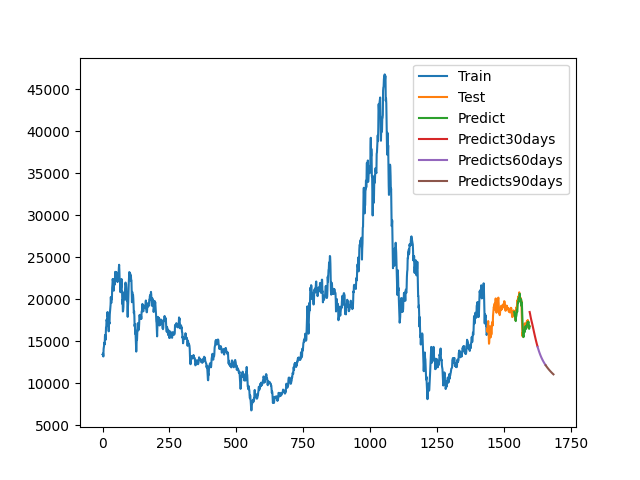
\includegraphics[width=1\textwidth]{experiment/ltsm/Team4_LSTM_DXG_9_1.png}
    \caption{LSTM DXG 9-1}
    \label{fig:nvl_histogram}
    \end{minipage}

    \begin{minipage}{0.23\textwidth}
    \centering
    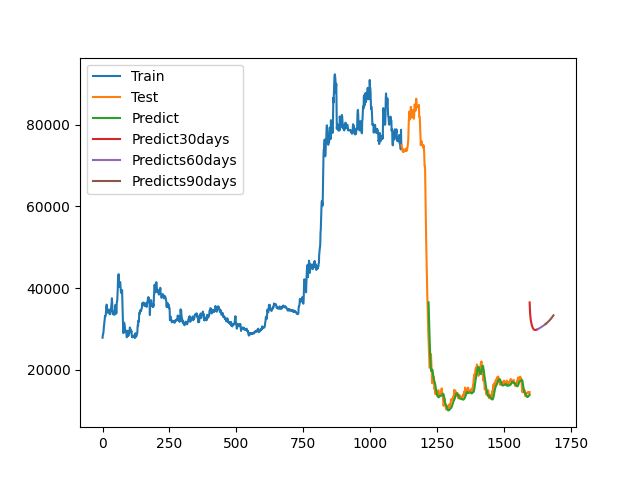
\includegraphics[width=1\textwidth]{experiment/ltsm/Team4_LSTM_NVL_7_3.png}
    \caption{LSTM NVL 7-3}
    \label{fig:nvl_boxplot}
    \end{minipage}
    \hfill
    \begin{minipage}{0.23\textwidth}
    \centering
    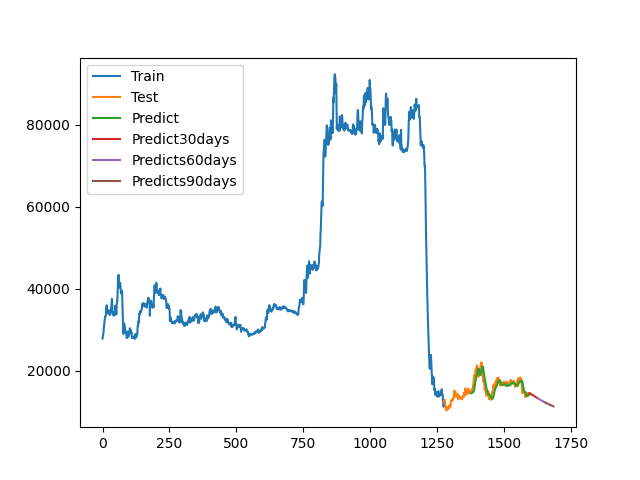
\includegraphics[width=1\textwidth]{experiment/ltsm/Team4_LSTM_NVL_8_2.png}
    \caption{LSTM NVL 8-2}
    \label{fig:nvl_histogram}
    \end{minipage}
    \begin{minipage}{0.23\textwidth}
    \centering
    \includegraphics[width=1\textwidth]{experiment/ltsm/Team4_LSTM_NVL_9_1.png}
    \caption{LSTM NVL 9-1}
    \label{fig:nvl_histogram}
    \end{minipage}
\end{figure}

\newpage

\section{Result}

\subsection{Model Evaluation with NVL Dataset}

\begin{table}[htbp]
\caption{7-3 Train-Test Ratio}
\begin{center}
\begin{tabular}{|c|c|c|c|}
\hline
\textbf{Evaluation}&\multicolumn{3}{|c|}{\textbf{Evaluation Metric}} \\
\cline{2-4} 
\textbf{Model} & \textbf{\textit{MAE}}& \textbf{\textit{MAPE}}& \textbf{\textit{RMSE}} \\
\hline
ETS & 10760.862 & 0.6269 & 12282.007\\
\hline
TBATS & 47834.0683981406 & 3.07015698344784 & 52333.6378114025\\
\hline
Kalman Filter & 248.39356236518 & 0.856696738701653 & 1555.81855814945\\
\hline
ResNet & 23998.6308 & 164.0565 & 25054.4035\\
\hline
\end{tabular}
\label{tab1}
\end{center}
\end{table}

\begin{table}[htbp]
\caption{8-2 Train-Test Ratio}
\begin{center}
\begin{tabular}{|c|c|c|c|}
\hline
\textbf{Evaluation}&\multicolumn{3}{|c|}{\textbf{Evaluation Metric}} \\
\cline{2-4} 
\textbf{Model} & \textbf{\textit{MAE}}& \textbf{\textit{MAPE}}& \textbf{\textit{RMSE}} \\
\hline
ETS & 12978.866 & 0.8054 & 13836.799\\
\hline
TBATS & 5735.10288615056 & 0.350508382672752 & 6267.97272700285\\
\hline
Kalman Filter & 139.208035812137 & 0.826768461381157 & 635.126921080275\\
\hline
ResNet & 1692.5887 & 9.6903 & 1916.3659\\
\hline
\end{tabular}
\label{tab1}
\end{center}
\end{table}

\begin{table}[htbp]
\caption{9-1 Train-Test Ratio}
\begin{center}
\begin{tabular}{|c|c|c|c|}
\hline
\textbf{Evaluation}&\multicolumn{3}{|c|}{\textbf{Evaluation Metric}} \\
\cline{2-4} 
\textbf{Model} & \textbf{\textit{MAE}}& \textbf{\textit{MAPE}}& \textbf{\textit{RMSE}} \\
\hline
ETS & 17005.866 & 0.9134 & 17005.799\\
\hline

TBATS & 4402,61355422372 & 0,265717832572438 & 4732,26345311019\\
\hline
Kalman Filter & 157.422364473748 & 0.865352442266032 & 781.529137493465\\
\hline
ResNet & 477.0171 & 3.0175 & 551.2267\\
\hline
\end{tabular}
\label{tab1}
\end{center}
\end{table}

\newpage

\subsection{Model Evaluation with DIG Dataset}

\begin{table}[htbp]
\caption{7-3 Train-Test Ratio}
\begin{center}
\begin{tabular}{|c|c|c|c|}
\hline
\textbf{Evaluation}&\multicolumn{3}{|c|}{\textbf{Evaluation Metric}} \\
\cline{2-4} 
\textbf{Model} & \textbf{\textit{MAE}}& \textbf{\textit{MAPE}}& \textbf{\textit{RMSE}} \\
\hline
ETS & 12978.866 & 0.8054 & 13836.799\\
\hline
TBATS & 9343.21964965822 & 0.510739796617613 & 10964.3189201992\\
\hline
Kalman Filter & 250.027658291219 & 1.14432132503519 & 656,424883089693\\
\hline
ResNet & 608.8179 & 2.9155 & 784.8124\\
\hline
\end{tabular}
\label{tab1}
\end{center}
\end{table}

\begin{table}[htbp]
\caption{8-2 Train-Test Ratio}
\begin{center}
\begin{tabular}{|c|c|c|c|}
\hline
\textbf{Evaluation}&\multicolumn{3}{|c|}{\textbf{Evaluation Metric}} \\
\cline{2-4} 
\textbf{Model} & \textbf{\textit{MAE}}& \textbf{\textit{MAPE}}& \textbf{\textit{RMSE}} \\
\hline
ETS & 12978.866 & 0.8054 & 13836.799\\
\hline
TBATS & 9896.61659039693 & 0.387781985119017 & 10921.9629974825\\
\hline
Kalman Filter & 189.295680805776 & 0.863106784469551 & 281.184875988358\\
\hline
ResNet & 721.7579 & 2.7584 & 937.6967\\
\hline
\end{tabular}
\label{tab1}
\end{center}
\end{table}

\begin{table}[htbp]
\caption{9-1 Train-Test Ratio}
\begin{center}
\begin{tabular}{|c|c|c|c|}
\hline
\textbf{Evaluation}&\multicolumn{3}{|c|}{\textbf{Evaluation Metric}} \\
\cline{2-4} 
\textbf{Model} & \textbf{\textit{MAE}}& \textbf{\textit{MAPE}}& \textbf{\textit{RMSE}} \\
\hline
ETS & 12978.866 & 0.8054 & 13836.799\\
\hline
TBATS & 5224.7253334245 & 0.186368637203841 & 5841.84259500596\\
\hline
Kalman Filter & 243.1862418430648 & 1.06414241847077 & 670.107588619744\\
\hline
ResNet & 1241.8686 & 4.1874 & 1407.7799\\
\hline
\end{tabular}
\label{tab1}
\end{center}
\end{table}

\newpage

\subsection{Model Evaluation with DXG Dataset}

\begin{table}[htbp]
\caption{7-3 Train-Test Ratio}
\begin{center}
\begin{tabular}{|c|c|c|c|}
\hline
\textbf{Evaluation}&\multicolumn{3}{|c|}{\textbf{Evaluation Metric}} \\
\cline{2-4} 
\textbf{Model} & \textbf{\textit{MAE}}& \textbf{\textit{MAPE}}& \textbf{\textit{RMSE}} \\
\hline
ETS & 12978.866 & 0.8054 & 13836.799\\
\hline
TBATS & 3866.19503802425 & 0.285752003979513 & 4856.4818828459\\
\hline
Kalman Filter & 128.100775541209 & 0.815818992436612 & 257.247713610622\\
\hline
ResNet & 727.179 & 4.9034 & 887.615\\
\hline
\end{tabular}
\label{tab1}
\end{center}
\end{table}

\begin{table}[htbp]
\caption{8-2 Train-Test Ratio}
\begin{center}
\begin{tabular}{|c|c|c|c|}
\hline
\textbf{Evaluation}&\multicolumn{3}{|c|}{\textbf{Evaluation Metric}} \\
\cline{2-4} 
\textbf{Model} & \textbf{\textit{MAE}}& \textbf{\textit{MAPE}}& \textbf{\textit{RMSE}} \\
\hline
ETS & 12978.866 & 0.8054 & 13836.799\\
\hline
TBATS & 6577.95858239967 & 0.374391057352586 & 7251.36610969733\\
\hline
Kalman Filter & 102.684117168683 & 0.644775423772767 & 161.435022499799\\
\hline
ResNet & 653.4036 & 3.6472 & 777.7216\\
\hline
\end{tabular}
\label{tab1}
\end{center}
\end{table}

\begin{table}[htbp]
\caption{9-1 Train-Test Ratio}
\begin{center}
\begin{tabular}{|c|c|c|c|}
\hline
\textbf{Evaluation}&\multicolumn{3}{|c|}{\textbf{Evaluation Metric}} \\
\cline{2-4} 
\textbf{Model} & \textbf{\textit{MAE}}& \textbf{\textit{MAPE}}& \textbf{\textit{RMSE}} \\
\hline
TBATS & 2968.83977645444 & 0.158792180656149 & 3259.94230073705\\
\hline
Kalman Filter & 109,986961845213 & 0,638855401653012 & 218.915199004979\\
\hline
ResNet & 462.8085 & 2.582 & 557.9483\\
\hline
\end{tabular}
\label{tab1}
\end{center}
\end{table}

\newpage

\section*{Acknowledgment}

% First and foremost, we would like to express our sincere gratitude to Assoc. Prof. Dr. Nguyen Dinh Thuan and Mr. Nguyen Minh Nhut for their exceptional guidance, expertise, and invaluable feedback throughout the research process. Their mentorship and unwavering support have been instrumental in shaping the direction and quality of this study. Their profound knowledge, critical insights, and attention to detail have significantly contributed to the success of this research. This research would not have been possible without the support and contributions of our mentors. We would like to extend our heartfelt thanks to everyone involved for their invaluable assistance, encouragement, and belief in our research. Thank you all for your invaluable assistance and encouragement.



\begin{thebibliography}{00}
\bibitem{b1} Hanke, J. E. (2008). Business Forecasting (Vol. 8). New Jersey:
Pearson Education International.
\bibitem{b2} Hyndman, R. J., Athanasopoulos, G. (2013). Forecasting:
Principles and Practice. Melbourne: OTexts
\bibitem{b3} Rim A., GiLang R. A., Sari S. W. Time series forecasting using exponential smoothing to predict the number of website visitor of Sebelas Maret University. (2015b, October 1). IEEE Conference Publication
\bibitem{b4} Alex Becker (www.kalmanfilter.net). (n.d.). Online kalman filter tutorial. https://www.kalmanfilter.net/multiSummary.html
\bibitem{b5}Perone, G. (2021). Comparison of ARIMA, ETS, NNAR, TBATS and hybrid models to forecast the second wave of COVID-19 hospitalizations in Italy. the European Journal of Health Economics, 23(6), 917–940. https://doi.org/10.1007/s10198-021-01347-4
\bibitem{b6}Time Series classification from scratch with Deep Neural Networks: A strong baseline | IEEE conference publication | IEEE Xplore, https://ieeexplore.ieee.org/abstract/document/7966039/ (accessed Jun. 6, 2024). 
\bibitem{b7}Short-term load forecasting based on Resnet and LSTM | IEEE Conference publication | IEEE Xplore, https://ieeexplore.ieee.org/abstract/document/8587554/ (accessed Jun. 6, 2024). 
\end{thebibliography}


\end{document}
